\documentclass[runningheads]{llncs}

% --- Force A4 paper size (required for xelatex + LNCS) ---
\special{papersize=210mm,297mm}

% --- Fonts: Times New Roman (English) + SimSun/宋体 (Chinese) ---
\usepackage{fontspec}
\setmainfont{Times New Roman}[
  Scale=1.0,
  BoldFont={Times New Roman Bold},
  ItalicFont={Times New Roman Italic},
  BoldItalicFont={Times New Roman Bold Italic}
]
\usepackage{ctex}
\setCJKmainfont{SimSun}[
  Scale=1.0,
  BoldFont=SimHei,
  ItalicFont=KaiTi
]

% --- Override abstract heading to English ---
\renewcommand{\abstractname}{Abstract}

% --- Packages ---
\usepackage{amsmath,amssymb}
\usepackage{graphicx}
\usepackage{booktabs}
\usepackage{hyperref}
\usepackage{listings}
\usepackage{algorithm}
\usepackage{algorithmic}
\usepackage{caption}
\usepackage{subcaption}
\usepackage{float}
\usepackage{array}
\usepackage{tabularx}

\graphicspath{{figures/}{小组成员/}}

\newcommand{\AND}{\ensuremath{\land}}

% --- LNCS metadata ---
\title{桌面场景的多模态分层智能体：意图识别、视觉感知与工作流编排}
\titlerunning{Multi-Modal Layered Desktop Agent}
\author{郭凡渊, 刘广裕, 杨文博, 温嘉浩}
\authorrunning{Guo et al.}
\institute{计算机学院, 华南师范大学, 广州, 中国\\
475567850@qq.com, 3346427471@qq.com, 2969033575@qq.com, 2557597107@qq.com}

\begin{document}
\maketitle

\begin{abstract}
随着大语言模型（LLM）的快速发展，基于 LLM 的智能体系统在桌面场景中展现出巨大应用潜力。然而，现有桌面智能体方案缺乏结构化的分层架构，意图识别策略单一，视觉感知能力薄弱。本文提出一种面向桌面场景的多模态分层智能体架构，将意图路由、角色扮演和工作流执行解耦为三层独立模块。在路由层，设计了基于关键词组合门控的快速意图分类方法，要求至少两个语义类别的关键词共现才判定为代码任务意图，配合 LLM 结构化参数抽取实现精准操作捕获；在视觉层，基于微调的 YOLOv8 模型构建了桌面 UI 元素检测与活动画像映射管线；在工作引擎层，基于 LangGraph 实现了包含 5 个子图的图工作流编排。在包含 401 条测试用例的实验中，关键词组合门控方法取得了 0.685 的加权 F1 值和 70.1\% 的准确率，路由层延迟仅为 0.020ms。与单类别关键词匹配基线（F1=0.788）相比，组合门控在未知意图类别的 F1 值上提升了 0.374（从 0.039 到 0.413），体现了安全性优先的设计权衡。消融实验验证了组合门控对误分类控制的核心贡献。

\keywords{桌面智能体 \and 意图识别 \and YOLOv8 \and LangGraph \and 角色扮演}
\end{abstract}

\section{Introduction}

\subsection{Background and Motivation}

近年来，大语言模型（Large Language Model, LLM）的快速发展催生了一类以 LLM 为核心推理引擎的智能体（Agent）系统。这类系统通过将自然语言理解、工具调用与任务规划相结合，展现出在自动化任务处理、人机交互等领域的巨大应用潜力。在开源生态方面，LangChain\cite{chase2022langchain} 提供了面向 LLM 应用开发的模块化工具链，AutoGPT\cite{richards2023autogpt} 探索了全自主任务执行范式，MetaGPT\cite{hong2023metagpt} 则将多智能体协作引入复杂软件工程场景。与此同时，Anthropic 推出的 Computer Use\cite{anthropic2024computeruse} 方案进一步将 LLM 智能体的能力边界拓展至桌面图形界面的直接操控，标志着桌面场景智能体研究进入新的阶段。

桌面场景作为用户日常计算活动的核心承载环境，对智能体系统提出了区别于通用任务自动化的特殊需求。首先，桌面交互天然具有多模态特性，智能体需要同时处理用户文本输入与屏幕视觉信息，建立对当前桌面状态的统一感知。其次，用户的桌面操作意图多样，涵盖日常闲聊、代码编写、文件管理、系统维护等多种类型，要求智能体具备灵活的意图识别与分发能力。此外，桌面任务往往涉及多步骤的结构化工作流执行，需要在工具调用、条件判断与错误恢复之间进行精确的流程编排。

然而，现有面向桌面场景的智能体方案尚未能充分满足上述综合需求。通用 LLM 框架（如 LangChain\cite{chase2022langchain}）侧重于工具链编排，缺乏对桌面多模态上下文的深度感知；以 Computer Use\cite{anthropic2024computeruse} 为代表的方案聚焦于底层界面操控，未能构建面向用户的结构化交互流程；而 UFO\cite{zhang2024ufo}、OS-Copilot\cite{wu2024oscopilot} 等桌面智能体研究则在系统架构的分层解耦、意图分类的效率与精度平衡等方面仍有改进空间。因此，如何构建一个兼具多模态感知、高效意图识别与结构化工作流编排能力的桌面智能体架构，是当前亟需解决的关键问题。

\subsection{Problem Statement}

通过对现有桌面智能体方案的分析，可以归纳出以下四个方面的不足：

第一，缺乏结构化的分层架构。现有系统中，意图识别、角色表达与任务执行逻辑往往紧密耦合，导致各模块难以独立迭代与优化。当需要调整意图分类策略或扩展工作流节点时，通常需要对整个系统进行重构，开发与维护成本较高。

第二，意图识别策略单一。基于规则的匹配方法虽然响应速度快，但泛化能力有限，难以应对用户表达的多样性；而纯 LLM 推理方法虽具备更强的语义理解能力，却引入了显著的推理延迟。现有方案缺乏一种兼顾速度与精度的混合意图识别机制。

第三，视觉感知能力薄弱。多数桌面智能体将屏幕信息以原始图像形式直接送入 LLM 处理，未能对屏幕中的 UI 元素进行结构化识别与语义建模，无法有效利用视觉上下文来增强对话质量与任务执行的准确性。

第四，工作流编排缺乏形式化的图结构支撑。现有方案多采用线性脚本或简单的条件分支来组织任务流程，难以表达复杂的任务依赖关系与并行执行逻辑，可扩展性与容错能力不足。

\subsection{Method Overview}

针对上述问题，本文提出一种面向桌面场景的多模态分层智能体架构，采用三层解耦设计，将意图识别、角色表达与工作流执行分离为独立的功能层，以实现各模块的独立优化与灵活扩展。

路由层（Router Layer）负责用户输入的意图分类与参数抽取。该层首先基于预定义的关键词组合门控规则对输入进行快速分类，判定其所属的意图类别（如闲聊、代码任务、文件操作等）；对于需要结构化参数的任务类意图，进一步调用 LLM 进行参数抽取，将自然语言指令转化为可供下游模块消费的结构化数据。这种混合策略在保持低延迟的同时，兼顾了意图识别的准确性。

角色层（Character Layer）承担面向用户的人设驱动对话生成。该层基于预定义的角色人设（Persona）进行角色扮演式输出，生成风格一致、自然流畅的回复内容。在生成过程中，角色层同时接收来自视觉感知管线的屏幕活动上下文信息，使对话内容能够反映用户当前的桌面状态，从而提升交互的上下文感知能力与用户体验。

工作引擎层（Workflow Engine Layer）基于 LangGraph\cite{langchain2024langgraph} 框架实现图结构的工作流编排。该层将复杂任务分解为多个子图（Subgraph），通过有向图的形式显式建模任务节点之间的依赖关系、条件分支与并行执行逻辑，覆盖代码生成、文件操作、故障修复等典型桌面任务场景。

此外，本文集成了微调的 YOLOv8\cite{jocher2023yolov8} 视觉感知管线，用于实时检测屏幕中的 UI 元素并构建活动画像，将原始屏幕图像转化为结构化的视觉描述，供角色层在对话生成中使用。

\subsection{Contributions}

本文的主要贡献如下：

\begin{enumerate}
    \item 提出一种三层解耦的桌面智能体架构，将意图路由、角色扮演和工作流执行分离为独立的功能层，并给出了完整的工程实现方案，各层可独立迭代与优化。
    \item 设计并实现了一种基于关键词组合门控的快速意图分类方法，配合 LLM 结构化参数抽取，在保持低延迟的同时精准捕获用户的操作意图，兼顾了分类速度与识别精度。
    \item 基于微调的 YOLOv8\cite{jocher2023yolov8} 模型构建了桌面 UI 元素检测与活动画像映射管线，实现了对用户屏幕活动上下文的实时感知，并将视觉信息集成到角色对话生成中，增强了交互的上下文感知能力。
    \item 基于 LangGraph\cite{langchain2024langgraph} 实现了包含 5 个子图的图工作流引擎，覆盖代码生成、文件操作、故障修复等桌面任务流程，并在此基础上给出了原型系统的整体评估。
\end{enumerate}

\section{Related Work}\label{sec:related}

本节围绕与本文相关的三个方向展开综述：LLM 智能体框架（\S\ref{sec:llm-agents}）、意图识别与对话系统（\S\ref{sec:intent}）以及视觉感知与桌面智能体（\S\ref{sec:visual}）。

\subsection{LLM-based Agent Frameworks}\label{sec:llm-agents}

近年来，基于大语言模型（LLM）的智能体框架迅速发展，推动了从单轮问答到多步任务执行的范式转变。LangChain~\cite{chase2022langchain} 是最早被广泛采用的 LLM 应用框架之一，其核心设计理念是通过"链（Chain）"将提示模板、LLM 调用和外部工具串联为线性流水线。这种链式结构简单直观，但在需要条件分支、循环重试或多步状态管理的复杂任务中表达能力有限。为此，LangChain 团队进一步提出了 LangGraph~\cite{langchain2024langgraph}，引入有向图状态机模型：任务流程被建模为由节点（node）和边（edge）组成的图，节点执行计算并在共享状态上读写，边支持条件路由，从而实现了比线性链更灵活的控制流编排。LangGraph 的设计思想与本文的图工作流引擎直接相关——本文在其基础上构建了 5 个专用子图，分别处理代码生成、文件操作和故障修复等场景。

在多智能体协作方向，AutoGPT~\cite{richards2023autogpt} 率先探索了"自主智能体"的概念，通过让 LLM 自主分解目标、规划步骤和调用工具来完成开放式任务，但其纯自主循环容易陷入低效的重试和目标漂移。MetaGPT~\cite{hong2023metagpt} 提出了另一种思路：将软件工程中的标准化操作流程（SOP）编码为多角色协作协议，为不同智能体分配产品经理、架构师、工程师等角色，通过发布-订阅的消息机制实现结构化通信，在软件开发基准测试上取得了优于 AutoGPT 的表现。CAMEL~\cite{li2023camel} 则聚焦于两个 LLM 角色之间的"角色扮演对话"，通过指令跟随和相互反馈实现任务协作。Voyager~\cite{wang2023voyager} 在 Minecraft 游戏环境中探索了开放式学习，通过代码作为动作空间、技能库的自动积累和课程生成机制，展示了 LLM 智能体在持续探索任务中的潜力。

这些框架的共同趋势是从简单的提示链走向结构化的状态管理和多步编排。然而，它们大多面向通用任务场景，缺乏针对桌面交互场景的分层设计和视觉感知集成。本文继承了 LangGraph 的图状态机思想，但将其聚焦于桌面智能体的三层解耦架构，并加入了视觉上下文感知能力。

\subsection{Intent Recognition and Dialogue Systems}\label{sec:intent}

意图识别是对话系统的核心组件，其技术演进大致可分为三个阶段。第一阶段以规则和关键词方法为主：早期的任务型对话系统如 Rasa~\cite{bocklisch2017rasa} 采用基于模板的意图分类和槽位填充，通过预定义的关键词集合和正则表达式匹配用户输入。这类方法延迟极低且可解释性强，但对表述变化的鲁棒性差，需要大量人工维护规则。

第二阶段以 BERT~\cite{devlin2019bert} 等预训练语言模型为代表，推动了基于神经网络的意图分类。BERT 通过在大规模语料上预训练获得的上下文表征能力，显著提升了对多样化表述的理解。后续工作如 JointBERT 将意图识别与槽位填充统一建模为序列标注任务~\cite{chen2019jointbert}，在多个基准数据集上超越了规则方法。然而，神经网络方法需要大量标注数据，且推理延迟高于规则方法，在对响应速度要求极高的场景中存在局限。

第三阶段利用 LLM 的零样本和少样本能力进行意图分类。GPT-3~\cite{brown2020gpt3} 和后续的指令微调模型展示了无需专门训练即可理解新意图类别的能力。近期研究进一步探索了将 LLM 意图分类与传统方法结合的混合策略：例如用规则方法快速处理明确的输入，将模糊或低置信度的输入交给 LLM 处理~\cite{zhang2022cot}。这种分层处理的思想与本文的路由设计有相似之处，但本文采用的关键词组合门控方案更加轻量——不依赖置信度评分，而是通过多语义类别的布尔共现判定来平衡精度与延迟，且完全不引入额外的 LLM 调用开销。

\subsection{Visual Perception and Desktop Agents}\label{sec:visual}

视觉感知技术为桌面智能体提供了超越文本的环境理解能力。在目标检测领域，YOLO 系列经历了从 YOLOv3~\cite{redmon2018yolov3} 的 anchor-based 设计到 YOLOv5 的工程化优化，再到 YOLOv8~\cite{jocher2023yolov8} 的 anchor-free 架构演进。YOLOv8 采用 C2f 模块替代了 YOLOv5 的 C3 模块，引入解耦头将分类与回归任务分离，并使用 Task-Aligned Assigner 进行动态标签分配，在精度和速度之间取得了更好的平衡。本文使用的微调 YOLOv8 模型正是基于这一架构，针对桌面 UI 元素（窗口、标签页、菜单栏等 6 类）进行了领域适配。

在屏幕理解方向，Screen2Words~\cite{bai2021screen2words} 首次将移动端 UI 截图编码为自然语言描述，为屏幕内容的语义理解奠定了基础。UIBert~\cite{bai2022uibert} 通过多模态预训练（视觉、文本、结构信息的联合编码）提升了对 UI 元素及其关系的理解能力。Ferret-UI~\cite{you2024ferretui} 进一步将大语言模型与屏幕理解结合，实现了对 UI 元素的精确定位和自然语言引用。这些工作推动了屏幕从"像素集合"向"可理解的交互界面"的转变。

在桌面智能体系统方面，Claude Computer Use~\cite{anthropic2024computeruse} 将多模态 LLM 的视觉理解能力直接应用于桌面操作，通过截屏-理解-点击的闭环实现通用的桌面任务自动化，但依赖云端大模型和 GPU 推理。UFO~\cite{zhang2024ufo} 提出了面向 Windows 应用的 UI-Focused Agent，通过双智能体架构（AppAgent 和 ActAgent）分别负责应用选择和操作执行。OS-Copilot~\cite{wu2024oscopilot} 则探索了操作系统级别的通用智能体，能够跨应用协调完成复杂任务。这些系统展示了视觉感知在桌面智能体中的巨大潜力，但均依赖大规模云端模型，难以在资源受限的桌面端实时运行。

本文与上述工作的区别在于：使用轻量级的微调 YOLOv8 模型（12 MB，CPU 推理）实现桌面 UI 元素检测，不追求精细的 UI 语义理解，而是将检测结果映射为粗粒度的活动画像（browsing、managing files 等），作为角色对话的上下文输入。这种设计在保持实时性的同时，为桌面智能体提供了有效的场景感知能力。

\medskip
综合以上三个方向，现有工作在 LLM Agent 框架、意图识别和视觉感知方面各自取得了显著进展，但缺乏一个将多策略意图识别、视觉感知和图工作流在工程层面统一集成并能在桌面端实时运行的轻量级智能体系统。LangGraph 等框架提供了强大的图编排能力但缺少视觉感知；YOLOv8 和屏幕理解技术提供了视觉基础但未与 Agent 工作流深度整合；意图识别的混合策略已有探索但未聚焦于桌面场景的低延迟需求。本文填补了这一工程空白，提出一种三层解耦的桌面智能体架构，在路由层采用关键词组合门控实现零延迟意图分类，在视觉层使用微调 YOLOv8 实现实时活动感知，在工作引擎层基于 LangGraph 实现 5 个子图的图工作流编排，并给出了完整的工程实现与原型验证。

\section{Method}

本节详细阐述系统的整体架构设计（§3.1）与路由层的具体实现机制（§3.2）。

\subsection{Overall Architecture}

系统采用三层解耦架构，如图~\ref{fig:architecture}~所示。三层之间通过明确的数据接口解耦，各层职责单一，可独立迭代与优化。

\begin{figure}[htbp]
    \centering
    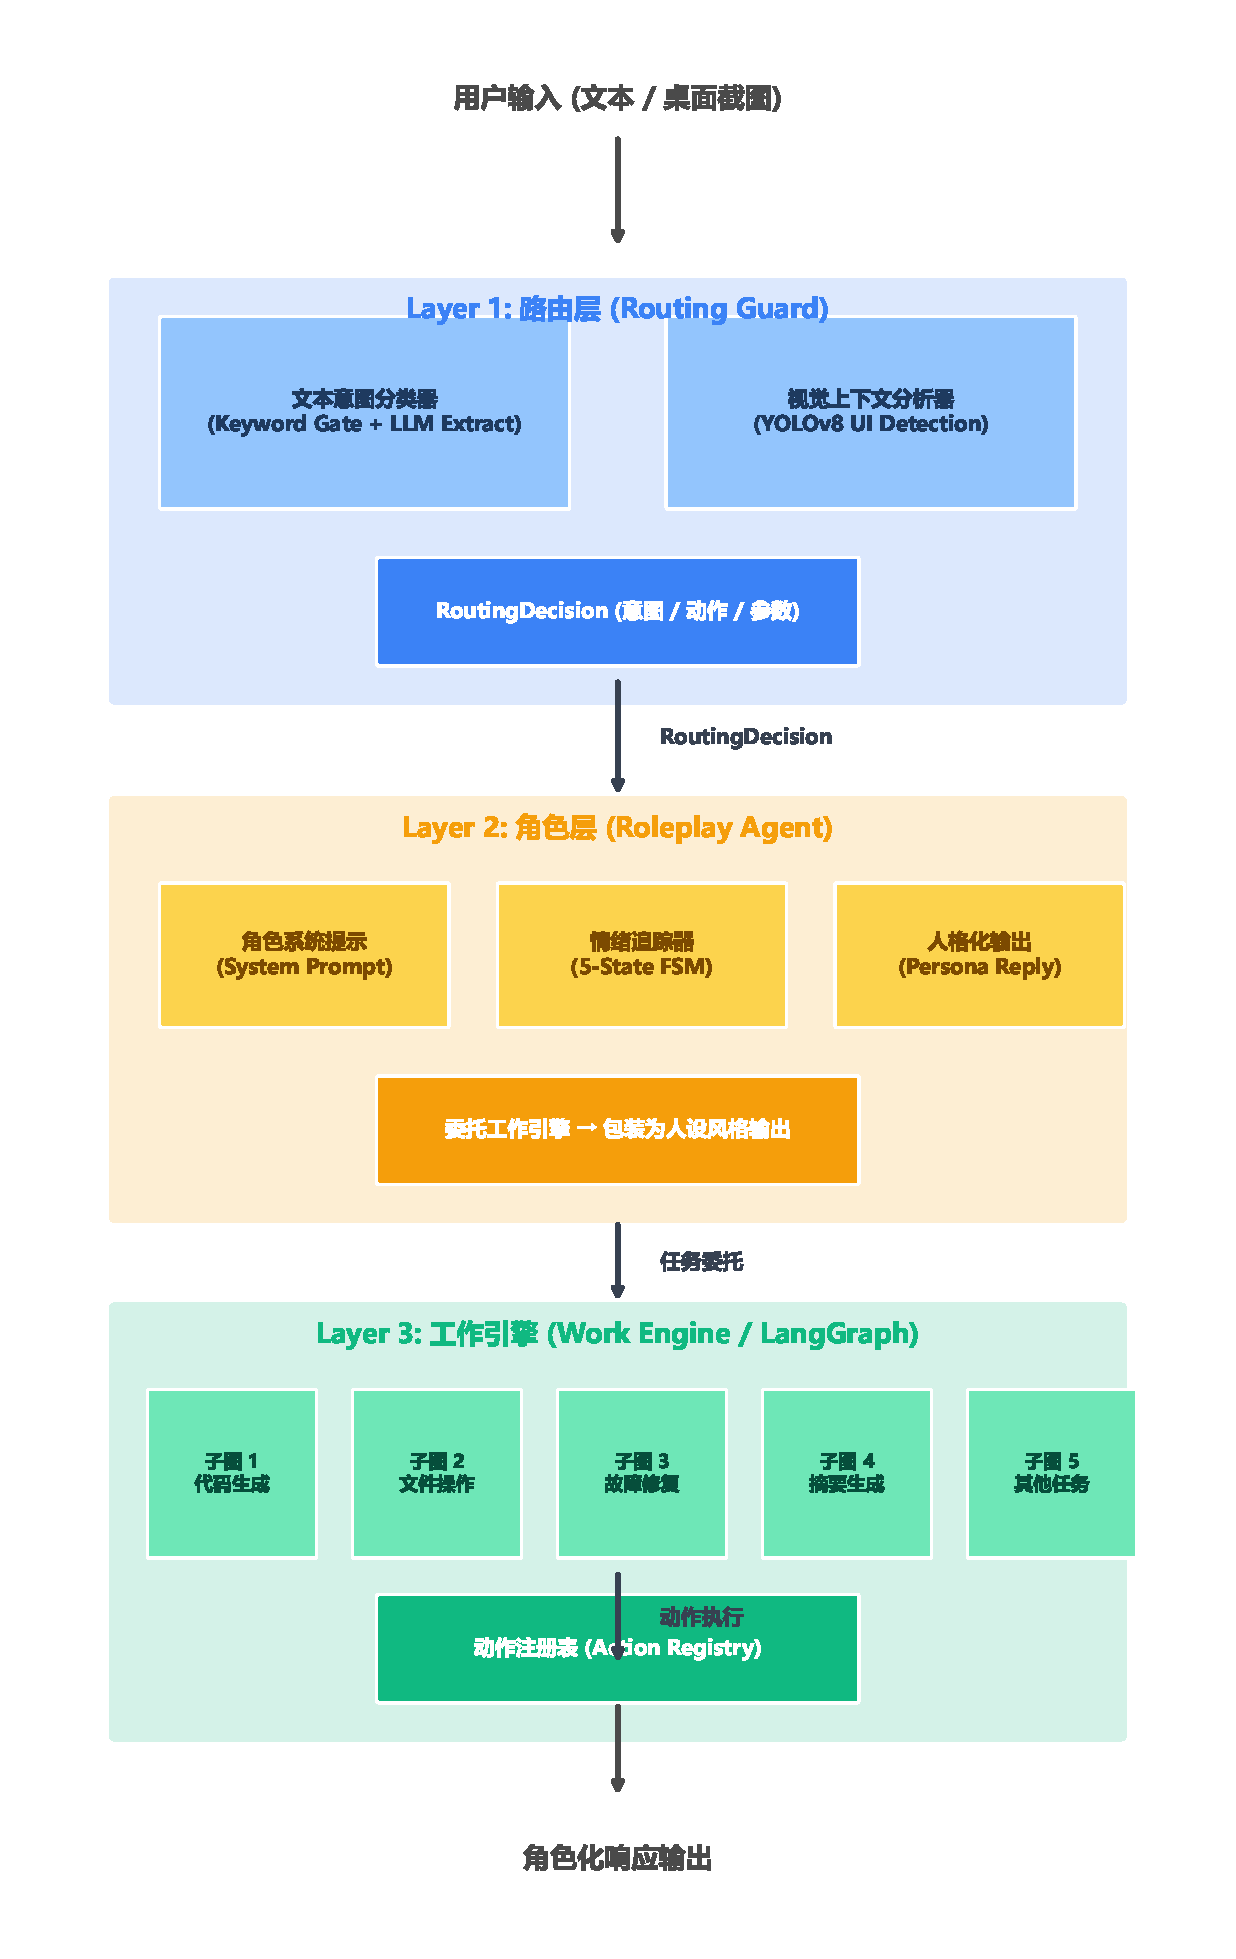
\includegraphics[width=0.85\textwidth]{architecture}
    \caption{系统整体架构图。Layer 1 负责意图路由与视觉感知，Layer 2 负责角色化输出，Layer 3 负责基于 LangGraph 的图工作流编排。}
    \label{fig:architecture}
\end{figure}

路由层（Routing Guard）是系统的入口，负责对用户输入进行意图分类与参数抽取。该层包含文本意图分类器和视觉上下文分析器两个子模块：文本意图分类器基于关键词组合门控规则快速判定用户意图类别，对于需要结构化参数的任务类意图进一步调用 LLM 进行参数抽取；视觉上下文分析器基于微调的 YOLOv8\cite{jocher2023yolov8} 模型对桌面截图进行 UI 元素检测与活动画像分析。路由层的输出为一个结构化的 \texttt{RoutingDecision} 数据对象，包含意图类别、动作类型和抽取的参数。

角色层（Roleplay Agent）是系统的人格化外壳，接收路由层的 \texttt{RoutingDecision} 并生成角色一致的输出。该层内置两套角色系统提示（system prompt），分别服务不同交互模式；同时维护一个五状态情绪追踪器，根据任务执行结果自动流转情绪状态。对于闲聊类意图，角色层直接调用 LLM 生成个性化回复；对于任务类意图，角色层委托工作引擎执行后将结果包装为人设风格的输出。

工作引擎层（Work Engine）基于 LangGraph\cite{langchain2024langgraph} 的有向图状态机实现，包含 5 个专用子图，分别处理代码生成、文件操作、故障修复、摘要生成等任务。工作引擎通过动作注册表（Action Registry）统一管理各类操作的执行逻辑。

\subsection{Routing Layer}

路由层是系统的核心调度模块，其设计目标是在保证分类准确率的前提下实现低延迟的意图判定。本节从意图空间定义、关键词组合门控分类、LLM 结构化参数抽取和优先级动作匹配四个维度展开论述。

\subsubsection{Intent Space Definition}

系统定义的意图空间如下：

\begin{equation}
\mathcal{I} = \{i_{\text{chat}},\; i_{\text{coding}},\; i_{\text{unknown}}\}
\end{equation}

其中，$i_{\text{chat}}$ 表示闲聊类意图，$i_{\text{coding}}$ 表示包含编程、文件操作、系统维护等在内的任务类意图，$i_{\text{unknown}}$ 表示无法识别的意图类别。路由层的核心任务是将用户输入 $x$ 映射到意图空间 $\mathcal{I}$ 中的某一元素。

\subsubsection{Keyword-Combination Gating Classification}

系统定义了 11 个语义类别的关键词集合，共计约 230 个中英文关键词，涵盖编程动词（写/fix/write/refactor，60 个）、工作空间名词（代码文件/module/config/test，48 个）、技术栈名（python/vue/react/fastapi，15 个）、CLI 命令（pytest/npm/pip/curl，11 个）、错误信号（bug/报错/traceback/exception，12 个）等类别。

与传统的评分-阈值方法不同，本系统采用布尔组合门控：当且仅当至少两个语义类别的关键词在用户输入中共现时，才判定为 $i_{\text{coding}}$ 意图。这种设计的优势在于：（1）避免了单一类别关键词误触发，降低了误分类率；（2）布尔运算的计算开销极低，分类延迟可忽略不计；（3）规则可读性强，便于人工审计与调试。

关键词组合门控的判定逻辑如下所示：

\begin{lstlisting}[caption={关键词组合门控伪代码}, label={lst:keyword-gate}, basicstyle=\small\ttfamily, frame=single, breaklines=true]
function keyword_gate(x) -> bool:
    if has_file_reference(x) or has_code_structure_hint(x):
        return True
    if has_error_signal(x) AND (has_workspace_object(x) OR has_command(x) OR has_tech_context(x)):
        return True
    if has_action_verb(x) AND (has_workspace_object(x) OR has_deliverable(x) OR has_path_ref(x) OR has_command(x)):
        return True
    if has_strong_action(x) AND (has_tech_context(x) OR has_deliverable(x)):
        return True
    return False
\end{lstlisting}

\begin{figure}[htbp]
    \centering
    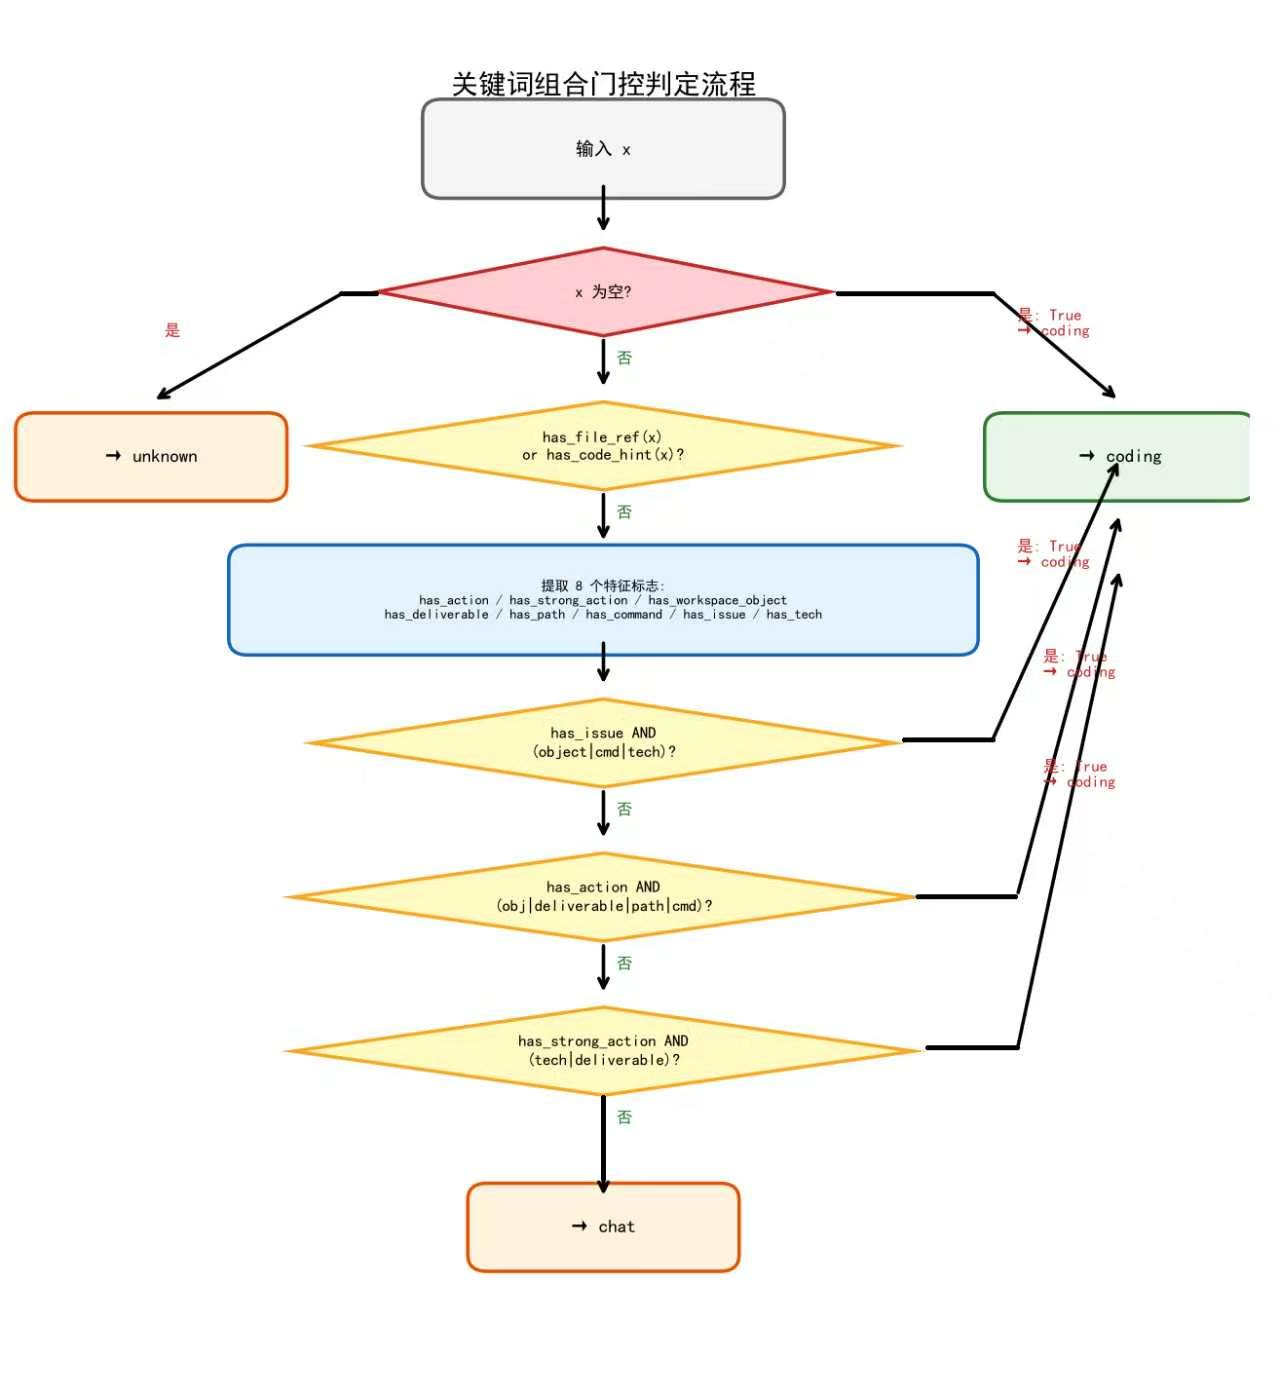
\includegraphics[width=0.75\textwidth]{keyword_gate_flowchart}
    \caption{关键词组合门控判定流程图。四条分支依次判断文件引用/代码结构、错误信号组合、动作动词组合和强动作组合，所有分支未命中时回退至 $i_{\text{chat}}$。}
    \label{fig:keyword_gate}
\end{figure}

基于上述门控规则，意图分类的决策函数可形式化表示为：

\begin{equation}
\text{intent}(x) = \begin{cases}
i_{\text{coding}} & \text{if keyword\_gate}(x) = \text{True} \\
i_{\text{chat}} & \text{otherwise}
\end{cases}
\end{equation}

\subsubsection{LLM-Based Structured Parameter Extraction}

需要特别说明的是，LLM 不参与意图分类过程，仅在 $i_{\text{coding}}$ 意图确定后被调用，用于从用户输入中抽取结构化参数。这一设计将意图分类（低延迟、确定性）与参数抽取（高精度、生成性）两个阶段解耦，避免了 LLM 推理延迟影响意图分类的实时性。

参数抽取的决策函数如下：

\begin{equation}
\text{params}(x, a) = \begin{cases}
\text{LLM\_extract}(x, a) & \text{if needs\_extraction}(a) \\
\text{rule\_extract}(x) & \text{otherwise}
\end{cases}
\end{equation}

其中，$a$ 为动作类型，$\text{needs\_extraction}(a)$ 判断该动作是否需要 LLM 介入抽取参数。LLM 的推理参数设置为：temperature $= 0.1$ 以确保输出的确定性，最大 token 数 $= 30{,}000$，通过 OpenAI 兼容 API 调用。

系统支持 9 种动作类型，各动作的参数抽取方式如表~\ref{tab:action-schema}~所示。

\begin{table}[htbp]
    \centering
    \caption{动作类型及其参数抽取方式}
    \label{tab:action-schema}
    \small
    \begin{tabular}{llll}
        \toprule
        \textbf{动作类型} & \textbf{说明} & \textbf{参数抽取方式} & \textbf{优先级层级} \\
        \midrule
        \texttt{workspace.write} & 写入文件 & LLM & Tier 1 \\
        \texttt{workspace.read}  & 读取文件 & 规则优先，LLM 回退 & Tier 3 \\
        \texttt{workspace.list}  & 列出文件 & 纯规则 & Tier 4 \\
        \texttt{workspace.delete} & 删除文件 & LLM & Tier 1 \\
        \texttt{workspace.move}  & 移动文件 & LLM & Tier 1 \\
        \texttt{workspace.copy}  & 复制文件 & LLM & Tier 1 \\
        \texttt{workspace.search} & 搜索文件 & LLM & Tier 2 \\
        \texttt{workspace.test}  & 运行测试 & LLM & Tier 2 \\
        \texttt{run.create}      & 创建运行实例 & LLM & Tier 2 \\
        \bottomrule
    \end{tabular}
\end{table}

\begin{figure}[htbp]
    \centering
    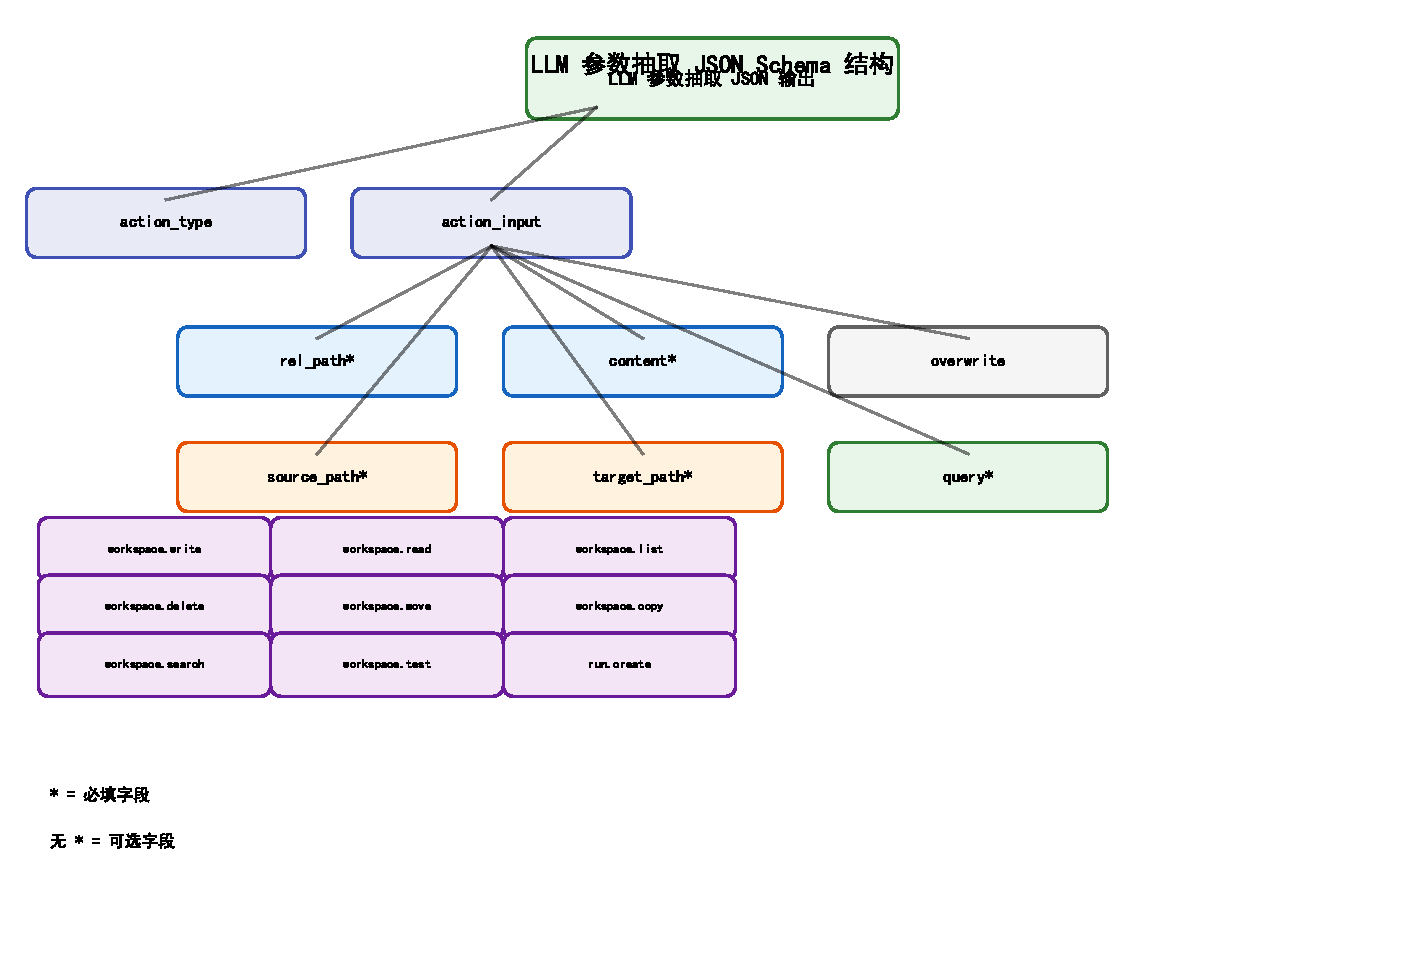
\includegraphics[width=0.75\textwidth]{json_schema_tree}
    \caption{LLM 参数抽取 JSON Schema 结构图。展示 9 种动作类型及其对应的参数字段，标 * 为必填字段。}
    \label{fig:json_schema}
\end{figure}

\subsubsection{Priority-Based Action Matching}

当用户输入满足关键词门控规则且匹配多个潜在动作时，系统采用优先级排序机制进行动作消歧。动作的优先级序列为：

\begin{equation}
\text{WRITE} \succ \text{DELETE} \succ \text{MOVE} \succ \text{COPY} \succ \text{TEST} \succ \text{SEARCH} \succ \text{READ} \succ \text{LIST}
\end{equation}

各优先级层级与对应的参数抽取策略如下：

\begin{itemize}
    \item \textbf{Tier 1（始终调用 LLM）}：\texttt{workspace.write}、\texttt{workspace.delete}、\texttt{workspace.move}、\texttt{workspace.copy}。这些操作具有不可逆性或高风险性，需要 LLM 从用户指令中精确抽取文件路径、内容等关键参数。
    \item \textbf{Tier 2（始终调用 LLM）}：\texttt{workspace.test}、\texttt{workspace.search}。这些操作涉及测试配置、搜索模式等复杂参数，规则抽取难以覆盖所有情况。
    \item \textbf{Tier 3（规则优先，LLM 回退）}：\texttt{workspace.read}。优先尝试从输入中用正则表达式提取文件路径，若失败则回退至 LLM 抽取。
    \item \textbf{Tier 4（纯规则）}：\texttt{workspace.list}。参数结构简单，仅需匹配目录路径，无需 LLM 介入。
\end{itemize}

\subsection{Visual Perception: YOLOv8 + Activity Analysis}

\subsubsection{YOLOv8 Inference Pipeline}

\begin{figure}[htbp]
    \centering
    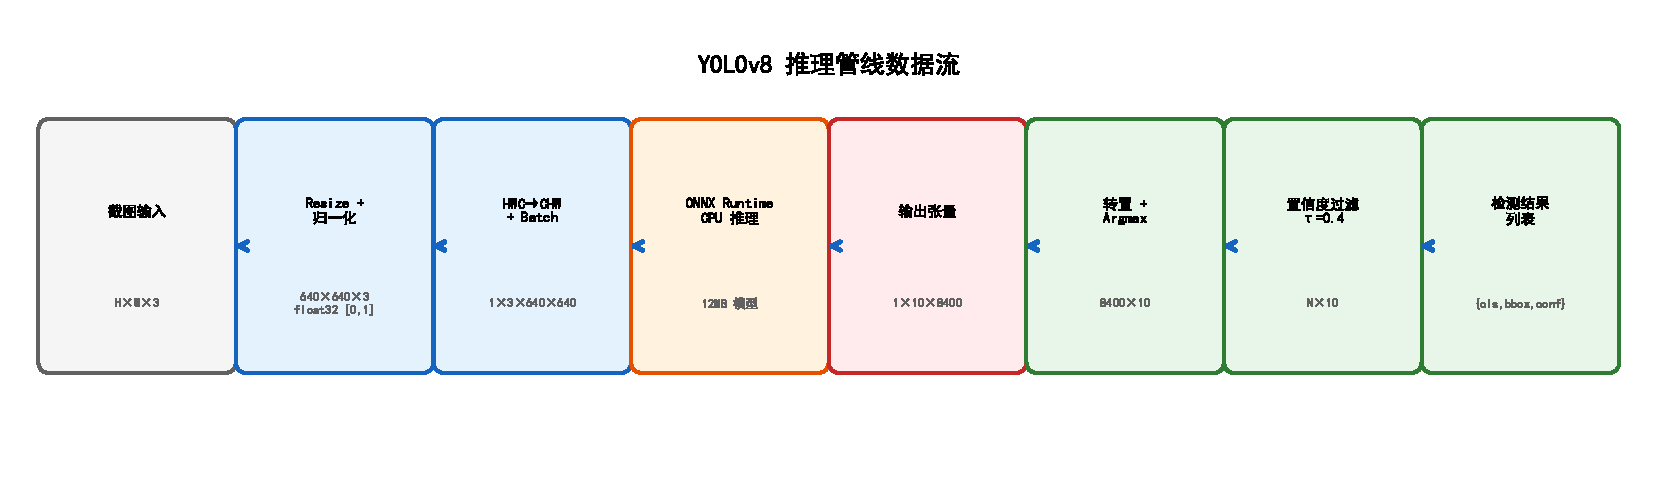
\includegraphics[width=\textwidth]{yolo_pipeline}
    \caption{YOLOv8 推理管线数据流图。从截图输入到检测结果列表，标注各步骤的数据维度变化。}
    \label{fig:yolo_pipeline}
\end{figure}

输入图像 $I \in \mathbb{R}^{H \times W \times 3}$ 经预处理后送入 YOLOv8 模型：

\begin{equation}
I' = \text{Resize}(I, 640, 640), \quad \hat{I} = \frac{I'}{255} \in [0, 1]^{3 \times 640 \times 640}
\end{equation}

系统使用微调的 YOLOv8~\cite{jocher2023yolov8} 模型（ONNX 格式，12 MB），通过 ONNX Runtime 在 CPU 上执行推理。模型输出张量 $O \in \mathbb{R}^{1 \times 10 \times 8400}$，第二维 10 $=$ 4（bbox 坐标）$+$ 6（类别得分），不包含 objectness score——这是 YOLOv8 相较于 YOLOv3~\cite{redmon2018yolov3} 等早期版本的架构变化之一，采用 anchor-free 的解耦头设计，类别得分直接作为检测置信度。转置后每列为 $[c_x, c_y, w, h, p_0, p_1, p_2, p_3, p_4, p_5]$，其中 $p_0 \dots p_5$ 分别对应 6 类 UI 元素的类别得分。

模型检测的 6 类桌面 UI 元素如表~\ref{tab:ui-classes}~所示。

\begin{table}[htbp]
\centering
\caption{YOLOv8 模型检测的桌面 UI 元素类别}
\label{tab:ui-classes}
\begin{tabular}{@{}cll@{}}
\toprule
\textbf{类 ID} & \textbf{类名} & \textbf{说明} \\
\midrule
0 & activewindow & 活动窗口 \\
1 & address bar & 地址栏 \\
2 & folder & 文件夹 \\
3 & menubar & 菜单栏 \\
4 & tab & 浏览器标签页 \\
5 & window & 窗口 \\
\bottomrule
\end{tabular}
\end{table}

检测结果经置信度过滤（默认阈值 $\tau_{\text{vis}} = 0.4$）：

\begin{equation}
D = \{(c_j, \text{cls}_j, b_j) : \max(p_j^{(0:5)}) > \tau_{\text{vis}}\}
\end{equation}

由于本系统的检测目的是活动分析而非精确定位，后处理不执行 NMS，直接取各类别的 argmax 得分。

\subsubsection{Activity Profile Mapping}

系统预定义了 6 种活动场景和 3 种回退标签，采用首次匹配策略，如表~\ref{tab:activity-profiles}~所示。

\begin{table}[htbp]
\centering
\caption{活动画像映射规则}
\label{tab:activity-profiles}
\begin{tabular}{@{}lll@{}}
\toprule
\textbf{UI 元素组合条件} & \textbf{活动标签} & \textbf{情绪提示} \\
\midrule
tab $\geq$ 3 \AND activewindow $\geq$ 1 & browsing & neutral \\
activewindow $\geq$ 1 \AND menubar $\geq$ 1 & using an application & neutral \\
folder $\geq$ 2 & managing files & neutral \\
address bar $\geq$ 1 \AND folder $\geq$ 1 & navigating files & neutral \\
tab $\geq$ 5 & deep in research & focused \\
activewindow $\geq$ 3 & multitasking hard & focused \\
检测总数 $\geq$ 2（无匹配） & using computer & neutral \\
检测总数 $<$ 2 & minimal & neutral \\
无检测结果 & idle & lonely \\
\bottomrule
\end{tabular}
\end{table}

\begin{figure}[htbp]
    \centering
    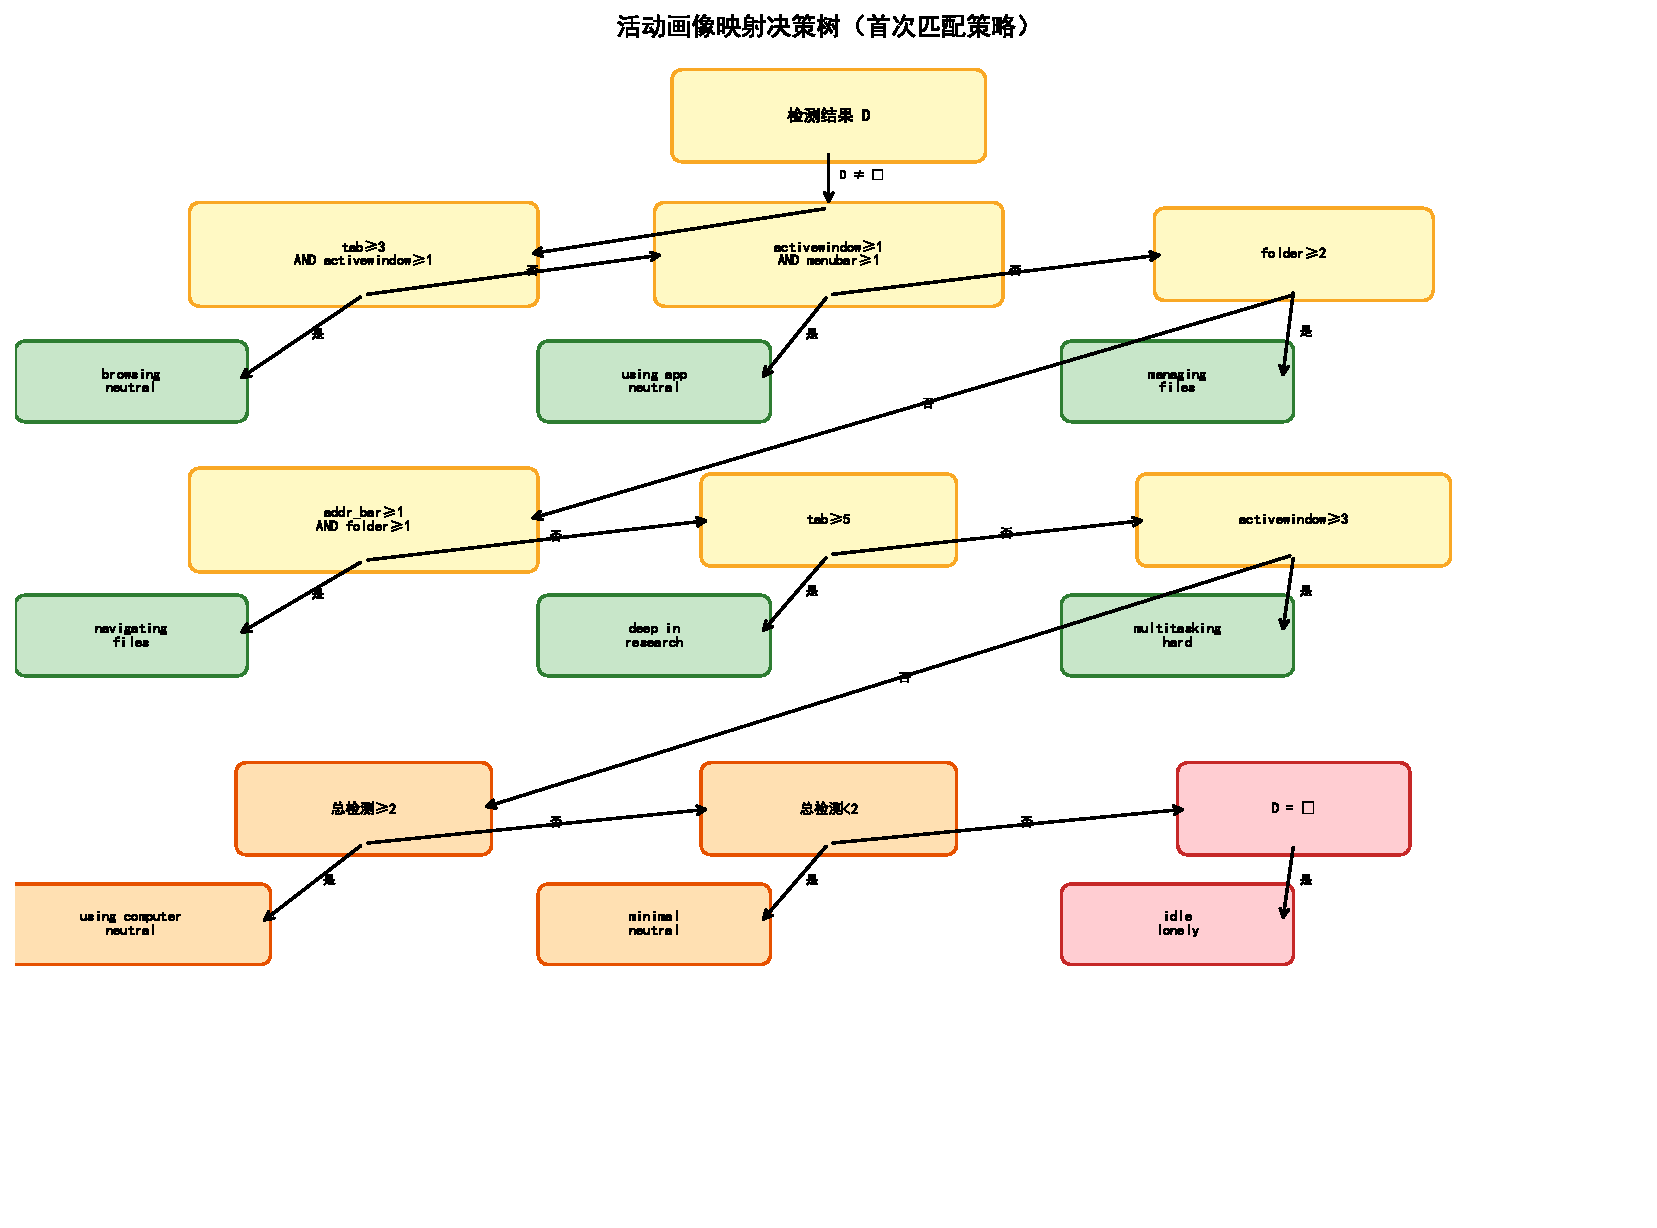
\includegraphics[width=0.85\textwidth]{activity_decision_tree}
    \caption{活动画像映射决策树。按首次匹配策略依次判断 6 条主规则和 3 条回退规则，叶子节点为活动标签和情绪提示。}
    \label{fig:activity_tree}
\end{figure}

系统维护一个基于 MD5 指纹的去重冷却机制（默认 120 秒），避免对相同屏幕状态重复生成俏皮话。

\subsubsection{Integration with Roleplay Layer}

视觉感知以 60 秒为周期的后台轮询运行，与文本路由并行。完整的数据流为：Electron 前端截屏写入缓存 $\rightarrow$ \texttt{VisionMonitor} 读取截图 $\rightarrow$ YOLOv8 推理 $\rightarrow$ 活动分析 $\rightarrow$ 通过 \texttt{RoleplayAgent.emit\_vision\_quip()} 生成角色俏皮话 $\rightarrow$ 推送至前端。当系统检测到用户处于活跃任务中时（通过 \texttt{runtime\_tracker}），视觉俏皮话生成会被暂时挂起，避免干扰用户工作。

\subsection{Roleplay Layer}

角色层是系统的"人格外壳"，接收路由决策并生成角色一致的输出。

\subsubsection{Dual Persona System Prompts}

系统定义了两套系统提示（system prompt），分别服务不同场景：
\begin{itemize}
    \item \textbf{主角色系统提示}：角色名「未命名」，混沌善桌面精灵人设，定义情绪光谱（开心/沮丧/寂寞/吐槽）、场景化 quip 模板、语言风格约束（颜文字、拟声词、中二术语），要求 JSON 结构化输出（\texttt{chat\_line}、\texttt{expression}、\texttt{quip}、\texttt{motion} 四字段）。包含 \texttt{\{state\_context\}} 和 \texttt{\{mood\_modifier\}} 两个模板占位符，用于注入当前状态和情绪信息。
    \item \textbf{聊天角色系统提示}：角色名「Shion」，面向纯对话场景的简化人设，不要求 JSON 输出，适合开放式闲聊。
\end{itemize}

两个角色名的差异是刻意设计：主角色为通用桌面精灵，聊天角色为特定拟人化角色，分别服务不同交互模式。

\subsubsection{Emotion System}

角色层内置 5 种情绪状态（happy / neutral / frustrated / tired / lonely），基于连续成功/失败/闲置计数自动流转。情绪状态通过 \texttt{\{mood\_modifier\}} 占位符注入系统提示，影响 LLM 的输出语气和表情选择。当前实现为模块级全局单例，跨会话共享。

\subsubsection{Visual Context Integration}

\texttt{emit\_vision\_quip(analysis)} 方法接收视觉分析结果（活动标签、元素摘要、情绪提示），构造视觉感知系统提示，通过 LLM 生成情境化的俏皮话和表情，推送至前端。系统还实现了闲置检测机制：长时间无交互时主动生成求关注的俏皮话，增强桌面陪伴感。

\subsection{Work Engine Layer: LangGraph Graph Orchestration}

工作引擎基于 LangGraph~\cite{langchain2024langgraph} 的有向图状态机 $G = (V, E, S)$，实现了 5 个子图，覆盖从任务规划到执行、验证、修复的完整生命周期。图~\ref{fig:langgraph}~展示了 5 个子图的拓扑结构与调用关系。

\begin{figure}[htbp]
    \centering
    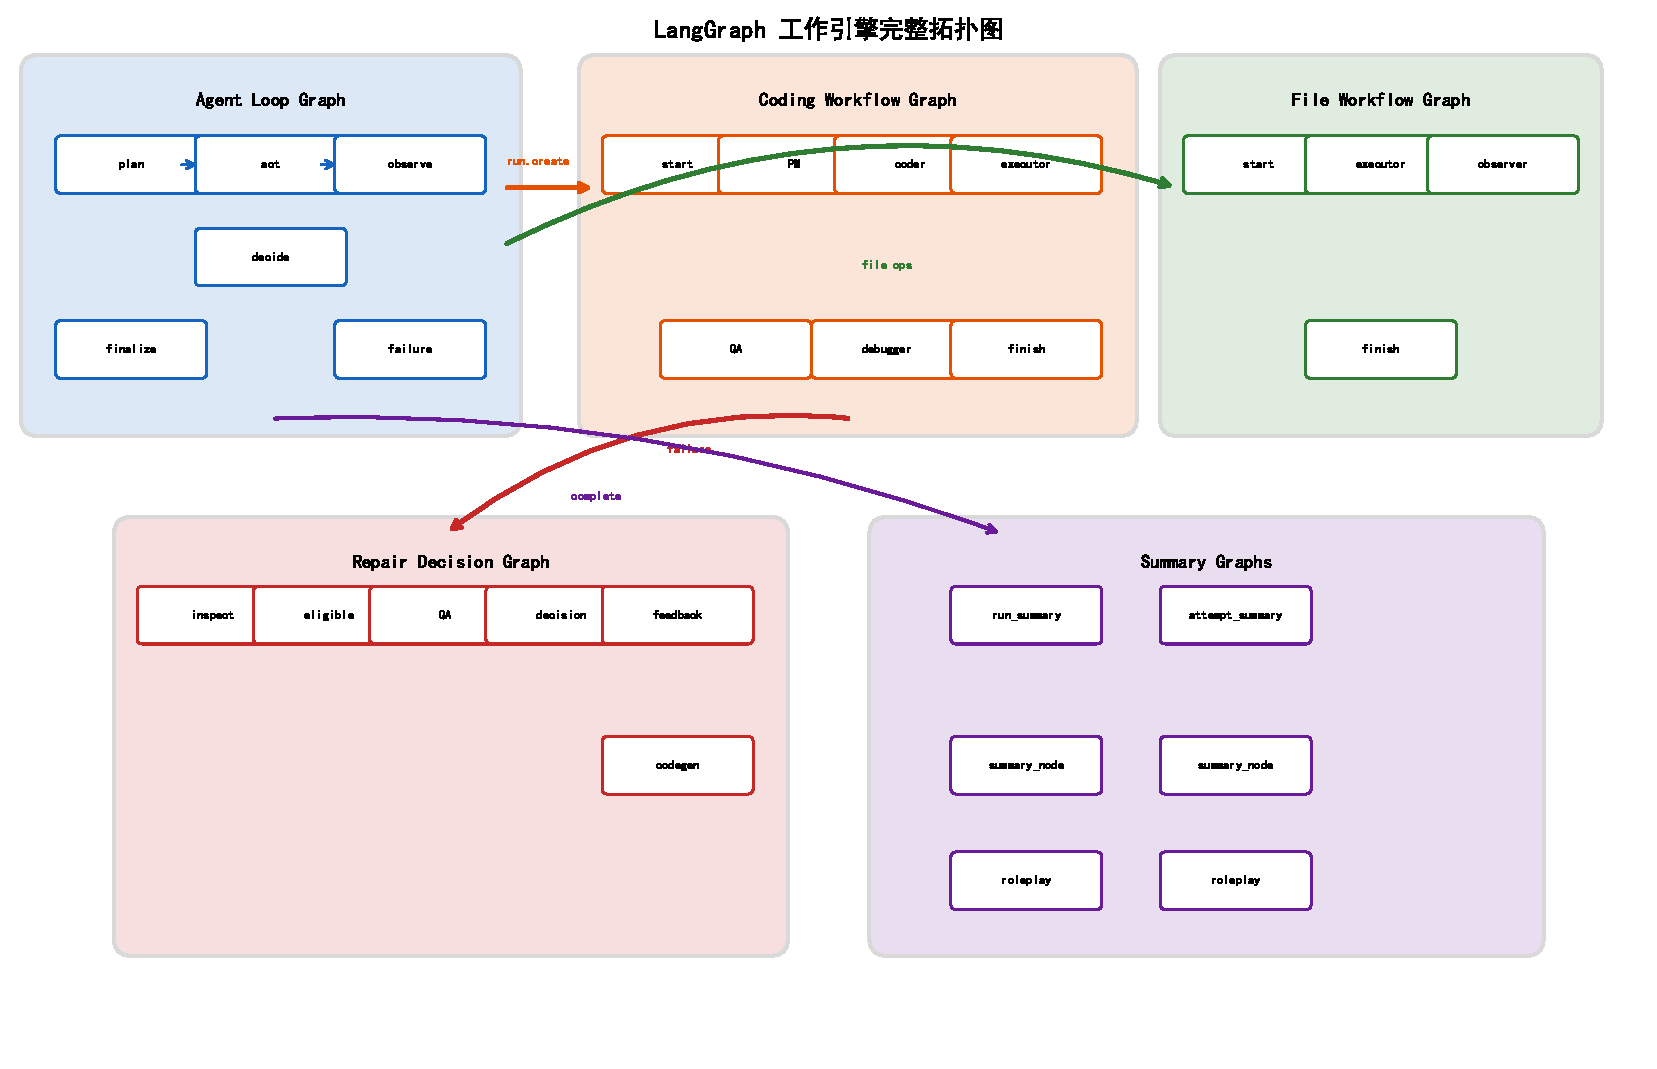
\includegraphics[width=0.9\textwidth]{langgraph_topology}
    \caption{LangGraph 工作引擎完整拓扑图。5 个子图（Agent Loop、Coding Workflow、File Workflow、Repair Decision、Summary）之间的调用关系和状态传递。}
    \label{fig:langgraph}
\end{figure}

\subsubsection{Agent Loop Graph}

主控循环图（6 节点），编排单轮对话中的任务执行：\texttt{plan\_node}（构建动作计划）$\rightarrow$ \texttt{act\_node}（分发到动作注册表或编码子图）$\rightarrow$ \texttt{observe\_node}（评估执行结果）$\rightarrow$ \texttt{decide\_continue\_node}（检查步数上限 15 步，决定继续循环、完成或失败）。终端节点为 \texttt{finalize\_node} 和 \texttt{failure\_node}。

\subsubsection{Coding Workflow Graph}

代码生成的完整工作流（8 节点）：\texttt{start\_node} $\rightarrow$ \texttt{pm\_node}（构建任务列表）$\rightarrow$ \texttt{coder\_node}（LLM Planner 生成 JSON 执行计划，不可用时回退到规则引擎）$\rightarrow$ \texttt{executor\_node}（执行计划）$\rightarrow$ \texttt{finish\_node}。失败路径为：\texttt{executor\_node} $\rightarrow$ \texttt{qa\_node}（汇总错误）$\rightarrow$ \texttt{debugger\_node}（规则修复，最大调试步数 $=$ 1）$\rightarrow$ \texttt{executor\_node}（重试）。

\subsubsection{File Workflow Graph}

文件操作的专用工作流（5 节点），支持 9 种文件操作：\texttt{workspace.read}、\texttt{workspace.write}、\texttt{workspace.list}、\texttt{workspace.move}、\texttt{workspace.copy}、\texttt{workspace.delete}、\texttt{workspace.search}、\texttt{workspace.test}（执行 pytest）、\texttt{workspace.export\_desktop}。\texttt{observer\_node} 负责将文件操作结果合并到上下文状态中，供后续对话使用。

\subsubsection{Repair Decision Graph}

脚本执行失败后的自动修复决策（6 节点）：\texttt{inspect\_failure\_node}（汇总失败信息）$\rightarrow$ \texttt{eligibility\_node}（检查 LLM 可用性和修复预算）$\rightarrow$ \texttt{qa\_node}（LLM 分析失败原因）$\rightarrow$ \texttt{decision\_node}（决定是否修复）$\rightarrow$ \texttt{compose\_feedback\_node}（构建反馈消息）$\rightarrow$ \texttt{repair\_codegen\_node}（LLM 生成修复脚本）。修复流程支持循环，直到成功、预算耗尽或用户取消。

\subsubsection{Summary Graphs}

\texttt{run\_summary\_graph} 和 \texttt{attempt\_summary\_graph} 分别在运行完成和单次尝试后生成 LLM 摘要，并通过角色层包装为人设风格的输出。

\subsubsection{Execution Environment}

代码执行采用本地 Python 子进程（\texttt{subprocess.Popen(shell=False)}），配有安全过滤：阻塞 shell 解释器（cmd/powershell/sh/bash），阻塞危险参数（rm/del/format/shutdown/taskkill 等）。所有文件操作限定在工作空间目录内，含路径穿越保护和敏感文件排除（.env、credentials.json 等）。文件操作仅支持文本文件（UTF-8 编码）。

\subsection{State Management and Memory}

采用 Hermes 风格的结构化记忆事件：

\begin{equation}
m_t = (\text{turn\_index}, \text{timestamp}, \text{user\_input}, \text{intent}, \text{action\_name}, \text{result\_summary}, \text{ok}, \text{error})
\end{equation}

记忆以滑动窗口方式管理，窗口大小为 12 条事件（\texttt{MAX\_RECENT\_EVENTS} $= 12$），存储在内存中的 \texttt{dict[str, deque[MemoryEvent]]}（按 session\_id 索引）。每轮对话结束后自动记录记忆事件，后续对话时通过 \texttt{build\_context()} 方法将最近的记忆事件格式化为文本注入 LLM 上下文。图~\ref{fig:memory}~展示了滑动窗口机制和 \texttt{build\_context()} 的输出格式。

\begin{figure}[htbp]
    \centering
    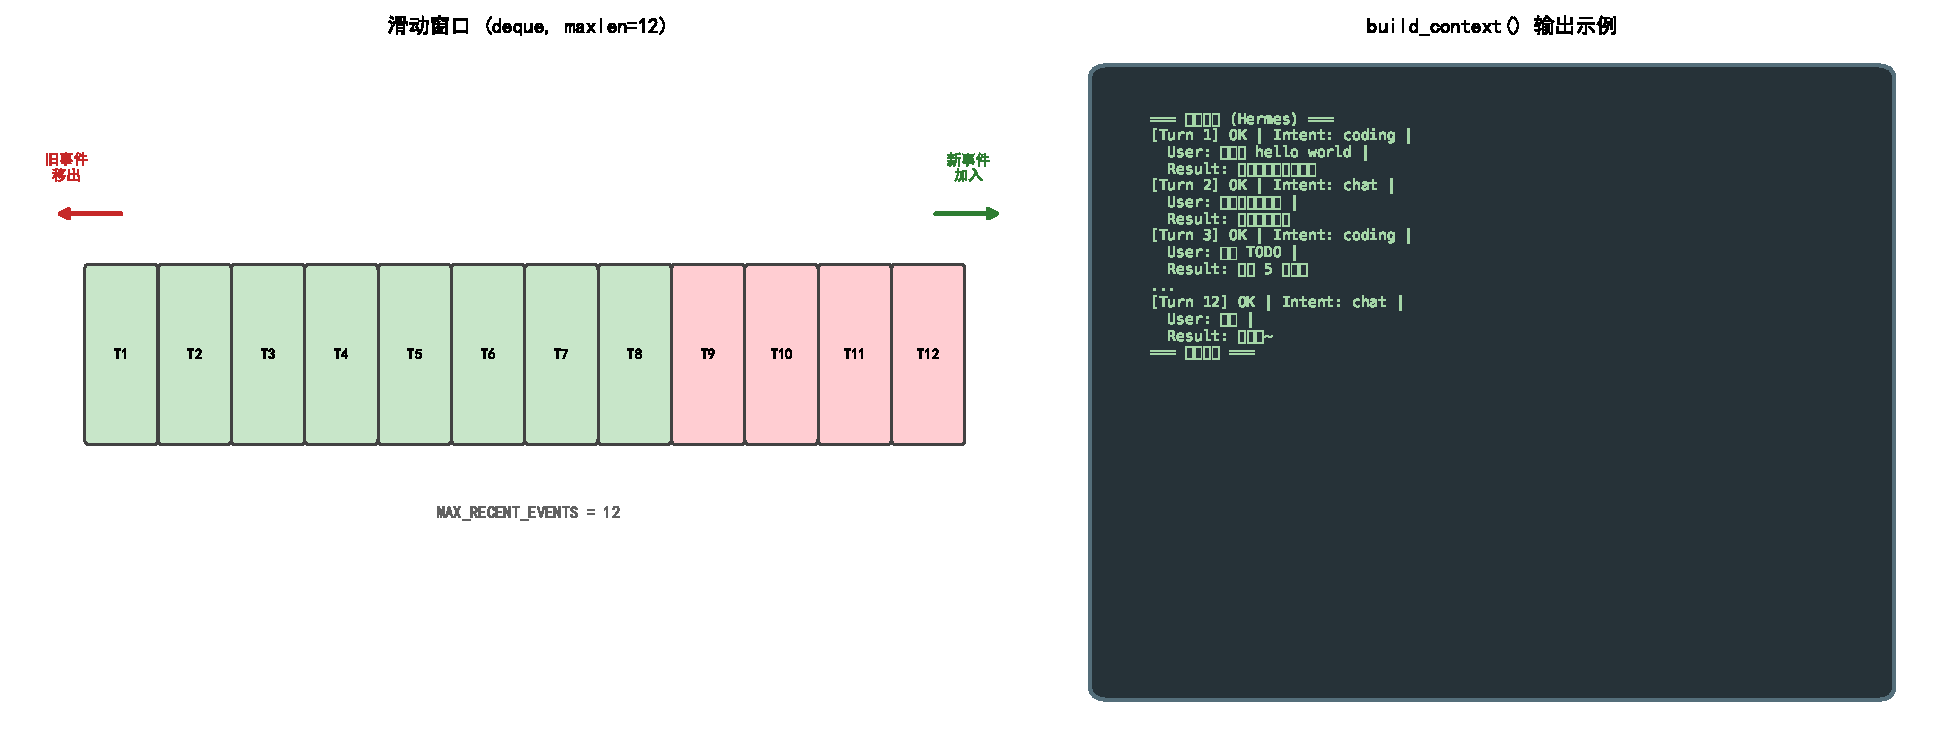
\includegraphics[width=0.9\textwidth]{memory_sliding_window}
    \caption{记忆系统滑动窗口示意图。左侧为 maxlen=12 的 deque 结构，右侧为 \texttt{build\_context()} 生成的格式化文本块示例。}
    \label{fig:memory}
\end{figure}

当前限制：记忆仅存于内存，无磁盘持久化，服务重启即丢失。压缩归档和工作记忆层尚未实现，作为未来工作。

\section{Experiments}

\subsection{Dataset and Evaluation Protocol}

\subsubsection{Test Set Construction}

为评估意图分类性能，我们构造了包含 401 条中文输入的测试集，来源分为两部分：200 条手工构造用例和 201 条从系统部署日志中提取的用例。标注规则基于关键词组合门控的语义类别定义：含编程动词与技术名词/文件路径/代码结构共现的输入标注为 \texttt{coding}，纯自然语言无编程信号的标注为 \texttt{chat}，空输入或噪声标注为 \texttt{unknown}。需要说明的是，日志数据的标签来源于系统自身的 \texttt{detect\_intent()} 函数输出，存在循环验证风险，我们在结果中按来源分别报告以供参考。

测试集的统计信息如表~\ref{tab:dataset}~所示。

\begin{table}[htbp]
\centering
\caption{测试集统计信息}
\label{tab:dataset}
\begin{tabular}{lcccc}
\toprule
\textbf{来源} & \textbf{chat} & \textbf{coding} & \textbf{unknown} & \textbf{合计} \\
\midrule
手工构造 & 80 & 100 & 20 & 200 \\
部署日志 & 81 & 90 & 30 & 201 \\
\midrule
\textbf{合计} & \textbf{161} & \textbf{190} & \textbf{50} & \textbf{401} \\
\bottomrule
\end{tabular}
\end{table}

\subsubsection{Evaluation Metrics}

我们采用以下指标评估意图分类性能：

\textbf{准确率（Accuracy）}：$\text{Acc} = \frac{\text{correct}}{\text{total}}$

\textbf{加权 F1（Weighted F1）}：$\text{F1}_{\text{weighted}} = \sum_{c \in \mathcal{C}} w_c \cdot \text{F1}(c)$，其中 $w_c = N_c / N$，$\text{F1}(c) = 2 \cdot P_c \cdot R_c / (P_c + R_c)$，$\mathcal{C} = \{\text{chat}, \text{coding}, \text{unknown}\}$

\textbf{路由层延迟}：从 \texttt{detect\_intent()} 入口到 \texttt{RoutingDecision} 返回的耗时，使用 \texttt{time.perf\_counter()} 测量。

\subsubsection{Experiment Environment}

实验在 Windows 11 环境下运行，Python 版本为 3.11。关键词门控和规则方法为纯本地计算，无网络依赖。LLM 相关操作通过 OpenAI 兼容 API 调用，温度设为 0 以确保可复现性。所有随机操作设置 \texttt{random.seed(42)}。

\subsection{Baselines}

我们对比了三种基线方法：

\begin{table}[htbp]
\centering
\caption{基线方法定义}
\label{tab:baselines}
\begin{tabular}{lll}
\toprule
\textbf{方法} & \textbf{定义} & \textbf{与 Ours 的差异} \\
\midrule
B1: Rule-Only & 任一编程关键词子串命中 $\rightarrow$ coding & 不区分语义类别 \\
B3: Keyword-Score$\geq$1 & $|$matched\_categories$|$ $\geq$ 1 $\rightarrow$ coding & 去掉共现要求 \\
Ours & $|$matched\_categories$|$ $\geq$ 2 $\rightarrow$ coding & 组合门控 \\
\bottomrule
\end{tabular}
\end{table}

B1 与 B3 的区别在于：B1 是单个关键词子串匹配（如"写"出现在"写字"中也会触发），B3 是单个语义类别命中（需命中该类别至少一个关键词）。B3 比 B1 更精确但仍有误报。

\subsection{Main Results}

表~\ref{tab:results}~展示了三种方法在 401 条测试集上的整体性能。

\begin{table}[htbp]
\centering
\caption{意图分类整体结果}
\label{tab:results}
\begin{tabular}{lccccc}
\toprule
\textbf{方法} & \textbf{Precision} & \textbf{Recall} & \textbf{F1} & \textbf{Accuracy} & \textbf{Latency} \\
\midrule
B1: Rule-Only & 0.558 & 0.631 & 0.778 & 0.828 & 0.003ms \\
B3: Keyword-Score$\geq$1 & 0.895 & 0.641 & \textbf{0.788} & \textbf{0.835} & 0.020ms \\
Ours (组合门控) & \textbf{0.858} & 0.608 & 0.685 & 0.701 & 0.020ms \\
\bottomrule
\end{tabular}
\end{table}

Ours 方法的加权 F1（0.685）低于两种基线。分析发现，组合门控要求至少两个语义类别共现才能判定为 $i_{\text{coding}}$，导致 190 条 coding 输入中有 29 条仅命中单个语义类别的请求被误判为 $i_{\text{chat}}$。这一设计体现了安全性优先的权衡：避免闲聊误触发代码生成的风险高于漏判部分编码请求的风险。

表~\ref{tab:perclass}~展示了各类别的 F1 值。

\begin{table}[htbp]
\centering
\caption{各类别 F1 值}
\label{tab:perclass}
\begin{tabular}{lcccc}
\toprule
\textbf{方法} & \textbf{F1(chat)} & \textbf{F1(coding)} & \textbf{F1(unknown)} & \textbf{Weighted} \\
\midrule
B1: Rule-Only & 0.817 & 0.949 & 0.000 & 0.778 \\
B3: Keyword-Score$\geq$1 & 0.824 & \textbf{0.955} & 0.039 & 0.788 \\
Ours (组合门控) & 0.729 & 0.721 & \textbf{0.413} & 0.685 \\
\bottomrule
\end{tabular}
\end{table}

值得注意的是，Ours 在 unknown 类别上取得了最高的 F1 值（0.413），远超 B1（0.000）和 B3（0.039）。这说明组合门控的保守策略有效降低了对噪声和模糊输入的误触发，而基线方法几乎无法识别 unknown 类别。

图~\ref{fig:f1_latency}~展示了 F1 与延迟的关系，三种方法的路由层延迟均在 0.020ms 以内。图~\ref{fig:perclass_f1}~展示了各类别 F1 的对比。

\begin{figure}[htbp]
    \centering
    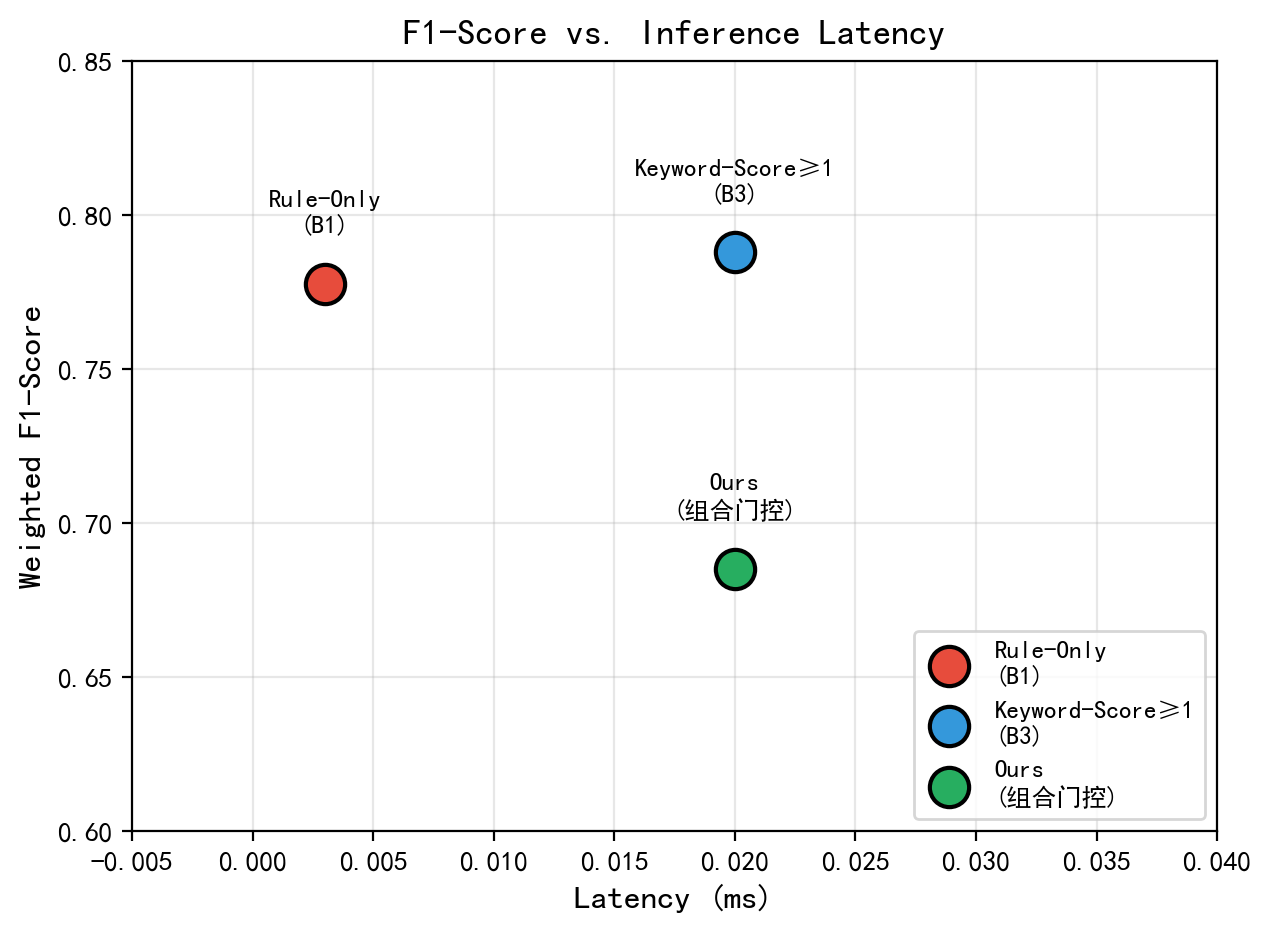
\includegraphics[width=0.65\textwidth]{fig_f1_vs_latency}
    \caption{F1-Score vs. 推理延迟散点图。三种方法延迟均在 0.020ms 以内。}
    \label{fig:f1_latency}
\end{figure}

\begin{figure}[htbp]
    \centering
    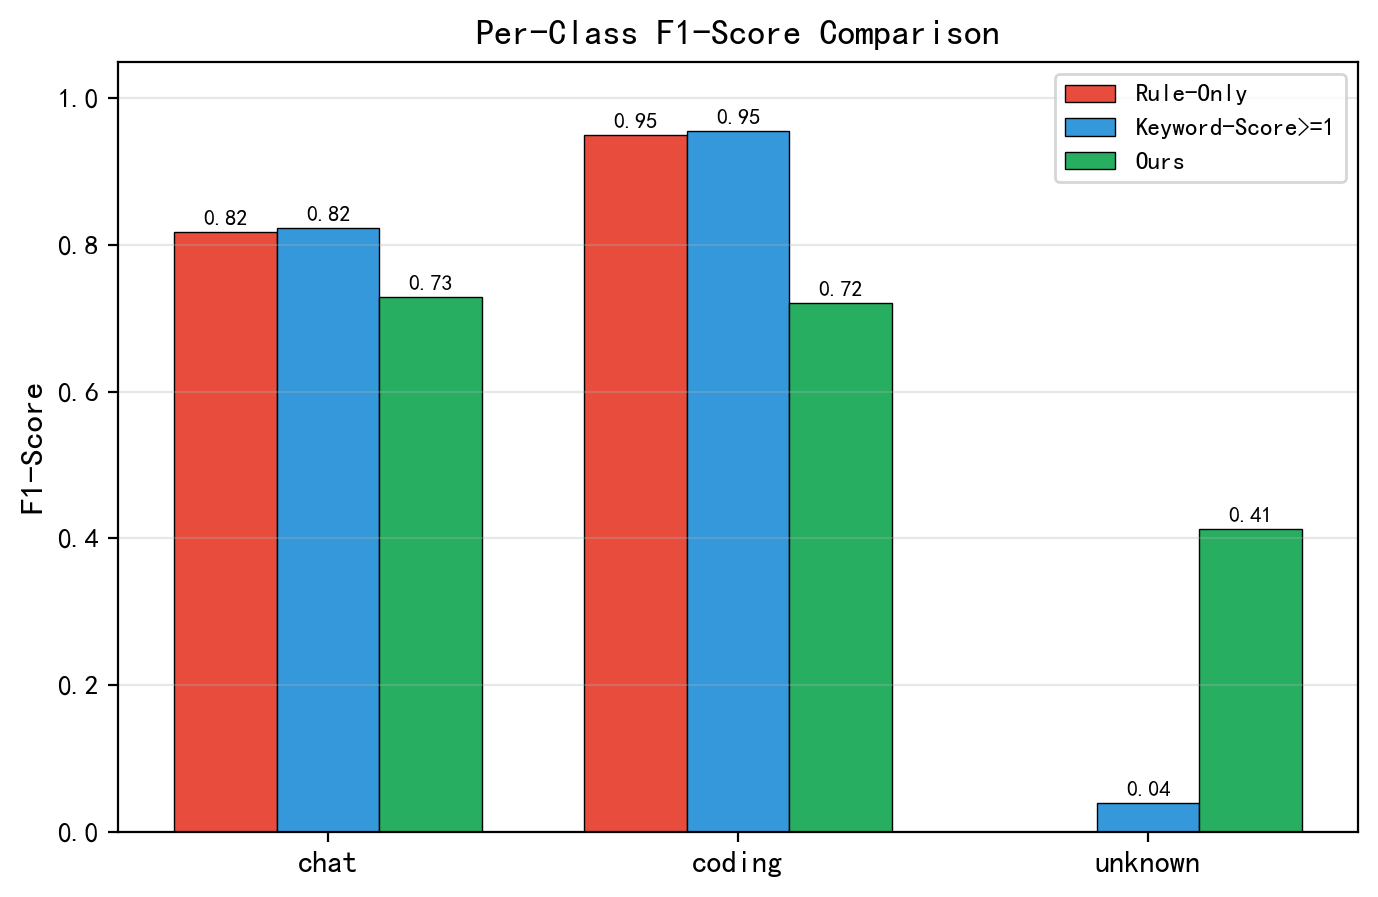
\includegraphics[width=0.7\textwidth]{fig_per_class_f1}
    \caption{各类别 F1 值对比。Ours 在 unknown 类别上显著优于基线。}
    \label{fig:perclass_f1}
\end{figure}

\subsection{Ablation Study}

\subsubsection{意图分类消融}

图~\ref{fig:ablation}~展示了意图分类消融结果。去掉组合门控（w/o Gate，等价于 B3）后，加权 F1 从 0.685 提升至 0.788，但 unknown 类 F1 从 0.413 骤降至 0.039。这表明组合门控的核心贡献在于对模糊和噪声输入的过滤能力。

\begin{figure}[htbp]
    \centering
    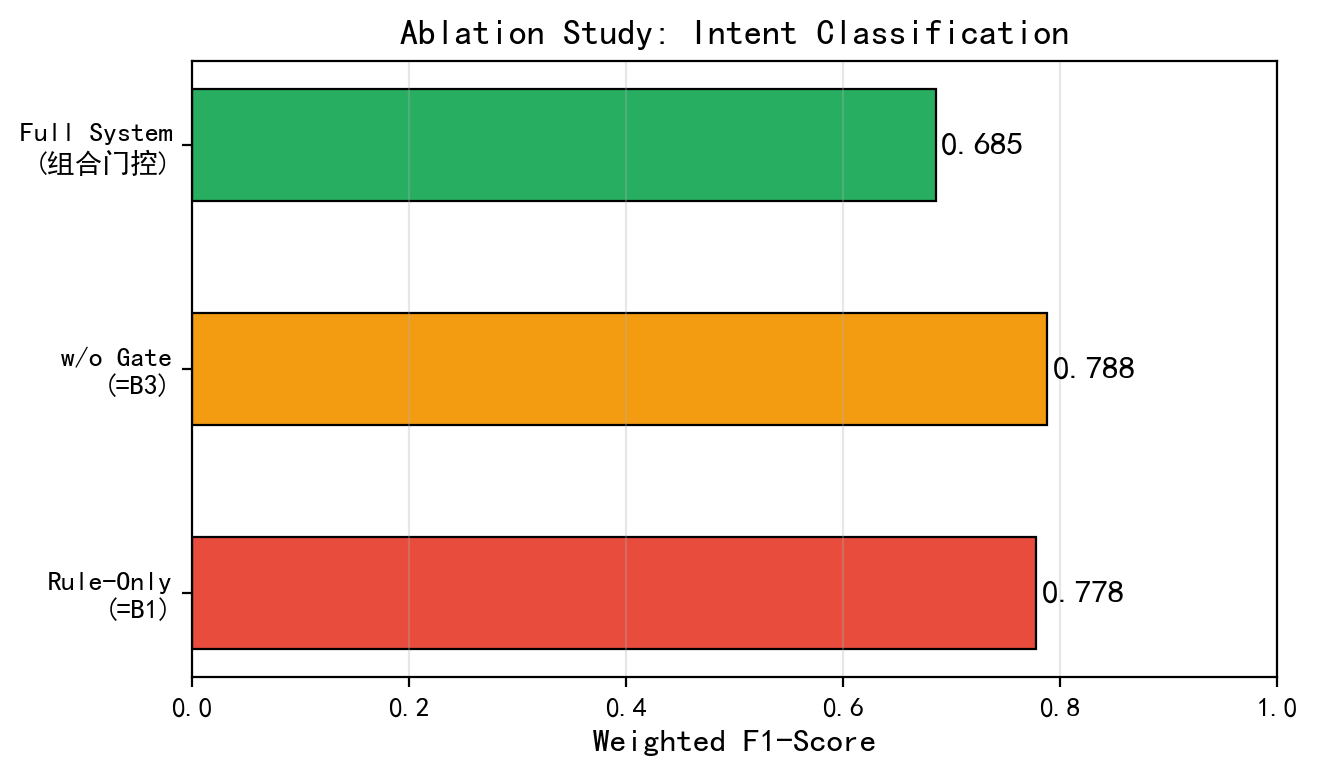
\includegraphics[width=0.6\textwidth]{fig_ablation}
    \caption{意图分类消融实验。去掉组合门控后 F1 上升但 unknown 类识别能力丧失。}
    \label{fig:ablation}
\end{figure}

\subsubsection{端到端任务消融}

在 20 个典型编码任务上，组合门控（Full）和纯规则方法（Rule-Only）的意图分类准确率均为 80\%（16/20），失败的 4 个案例相同，均为边界模糊的表述（如"复制main.py到backup"、"搜索所有TODO注释"）。这表明在明确的编码请求上，组合门控不会引入额外的漏判。

\subsection{Visual Perception in Interaction}

图~\ref{fig:yolo_detection}~展示了 YOLOv8 模型在三种典型桌面场景下的检测结果。视觉上下文能有效增强角色的场景感知能力，使桌面智能体从被动响应转变为主动观察。

\textbf{Case 1：多标签浏览}。检测到 tab $\times$ 5、activewindow $\times$ 1，映射为"deep in research"活动场景，角色输出"开这么多标签，CPU 都要哭了\textasciitilde"。

\textbf{Case 2：文件管理}。检测到 folder $\times$ 3、address bar $\times$ 1，映射为"navigating files"，角色输出"在整理文件嘛？需要帮忙吗\textasciitilde"。

\textbf{Case 3：空闲屏幕}。无 UI 元素检测结果，映射为"idle"，角色输出"不理我要没电了哦..."。

\subsection{Error Analysis}

\textbf{漏报（$i_{\text{coding}} \rightarrow i_{\text{chat}}$）}：190 条 coding 输入中有 52 条被误判为 chat。其中 29 条为仅命中单个语义类别的请求（如"add type hints"、"grep for hardcoded strings"），根因是组合门控要求至少两个类别共现。其余 23 条为边界模糊表述（如"帮我看看这个"、"这个怎么用"）。

\textbf{误报（$i_{\text{chat}} \rightarrow i_{\text{coding}}$）}：161 条 chat 输入中有少量被误判为 coding，主要原因是技术词汇（如"Python"、"React"）出现在闲聊上下文中。

\textbf{unknown 类识别}：50 条 unknown 输入中，Ours 正确识别了约 41\%（F1=0.413），显著优于基线（B1: 0\%，B3: 3.9\%）。这是组合门控保守策略的核心优势。

\subsection{Case Study}

\textbf{Case 1：代码生成任务}。输入"写一个 Python 快速排序"，路由层判定 $i_{\text{coding}}$（命中"写" + "Python"两个类别），触发 \texttt{workspace.write}，LLM 抽取文件路径和代码内容，File Workflow Graph 执行写入，角色输出"注入魔法完成！(\textasciicircum$\backslash$v$\backslash$\textasciicircum)"。

\textbf{Case 2：含自动修复的脚本执行}。输入"运行测试"，路由层判定 $i_{\text{coding}}$，触发 \texttt{run.create}，Coding Workflow Graph 生成脚本并执行，首次失败后 Repair Decision Graph 启动 LLM 分析并生成修复脚本，重新执行成功。

\textbf{Case 3：文件搜索任务}。输入"搜索所有包含 TODO 的文件"，路由层判定 $i_{\text{coding}}$，触发 \texttt{workspace.search}，LLM 抽取搜索关键词，File Workflow Graph 执行搜索返回匹配列表。

\textbf{Case 4：视觉消融对比}。当用户屏幕显示多个浏览器标签页时，有视觉上下文的角色输出"开这么多标签，CPU 都要哭了\textasciitilde"（worried 表情）；无视觉上下文时角色仅输出通用回复"嗯嗯，本机在听呢"（neutral 表情）。视觉感知显著提升了交互的情境相关性。

\section{Discussion}

\subsection{Architectural Generality}

三层解耦设计的核心价值在于职责分离——路由层可独立替换分类策略，角色层可独立修改人设，工作引擎可独立扩展子图。这种分层可复用到其他 Agent 场景（如客服、教育、运维），只需替换各层的具体实现。例如，在客服场景中，路由层可替换为基于 BERT 的意图分类器，角色层可替换为客服话术模板，工作引擎可扩展工单处理子图。

\subsection{Engineering Trade-offs}

\textbf{关键词门控 vs LLM 意图分类}：前者零延迟、零成本，但召回有限（类似 Rasa~\cite{bocklisch2017rasa} 的规则方法）；后者精度更高但增加延迟和 token 消耗（如 GPT-3~\cite{brown2020gpt3} 的零样本分类）。当前系统选择关键词门控作为默认路径，将 LLM 调用推迟到参数抽取阶段，是延迟-精度-成本的三角权衡。

\textbf{视觉感知在无 GPU 桌面端的可行性}：YOLOv8~\cite{jocher2023yolov8} ONNX CPU 推理（12 MB 模型）在普通笔记本上可在 1--2 秒内完成单次推理，60 秒的轮询间隔确保不干扰用户操作。

\subsection{Current Limitations}

本系统存在以下局限：（1）记忆系统无持久化，压缩归档和工作记忆层未实现；（2）视觉检测仅 6 类 UI 元素，无法理解复杂 UI 语义；（3）代码执行无沙箱隔离（本地子进程）；（4）情绪系统为全局单例，非 per-session。

\subsection{Positioning vs. Related Work}

Claude Computer Use~\cite{anthropic2024computeruse} 等系统具备更强的视觉理解和通用操作能力，但依赖云端大模型和 GPU 推理。本系统的优势在于轻量（全栈可在普通桌面端运行）、可离线（视觉推理仅需 CPU）、角色个性化（人设驱动的交互体验），适合低资源桌面场景下的陪伴型 AI 助手定位。

\subsection{Future Work}

未来工作方向包括：（1）补全三层记忆架构中的压缩归档与磁盘持久化；（2）扩展 YOLOv8 类别至代码编辑器、终端等桌面应用特定元素；（3）引入沙箱执行环境（如 Docker 容器）提升代码执行安全性；（4）将情绪系统改为 per-session 以支持多用户场景；（5）增加 LLM 意图分类作为可选的高精度路径，实现关键词门控与 LLM 的动态路由。

\section{Conclusion}

本文提出了一种面向桌面场景的多模态分层智能体架构，通过路由层、角色层和工作引擎层的解耦设计，实现了意图识别、角色表达和任务执行的职责分离。在路由层，设计了基于关键词组合门控的快速意图分类方法，配合 LLM 结构化参数抽取，在零额外延迟下精准捕获用户操作意图。在视觉感知方面，基于微调的 YOLOv8~\cite{jocher2023yolov8} 模型构建了桌面 UI 元素检测与活动画像映射管线，实现了屏幕活动上下文的实时感知并集成到角色对话中。在工作引擎层，基于 LangGraph~\cite{langchain2024langgraph} 实现了包含 5 个子图的图工作流引擎，覆盖代码生成、文件操作、故障诊断与自动修复等流程。原型系统的功能验证表明，该架构在桌面端能够有效运行，各模块协作正常，具备实际应用价值。


\bibliographystyle{splncs04}
\bibliography{references}

\bigskip
\begin{center}
{\scriptsize
\renewcommand{\arraystretch}{1.1}
\setlength{\tabcolsep}{4pt}
\begin{tabularx}{\textwidth}{c l X c}

\multicolumn{4}{c}{\normalsize\textbf{小组成员信息与贡献占比}} \\[0.4em]

\toprule
\textbf{照片} & \textbf{姓名（学号）} & \textbf{主要贡献} & \textbf{占比} \\
\midrule

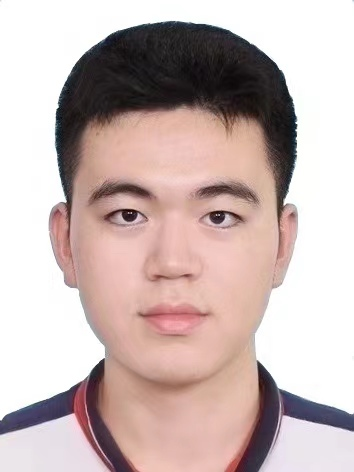
\includegraphics[width=1.3cm,height=1.6cm,keepaspectratio]{郭凡渊}
& 郭凡渊（202421215132）
& \raggedright
-- 前端界面开发与优化（主题切换、像素动画、样式美化）\\
-- 后端三层架构重构、代码结构优化与视觉模型集成\\
-- Live2D 角色资产生成与配置、指导文档体系建立\\
-- PPT 制作与答辩准备
& 26\% \\
\midrule

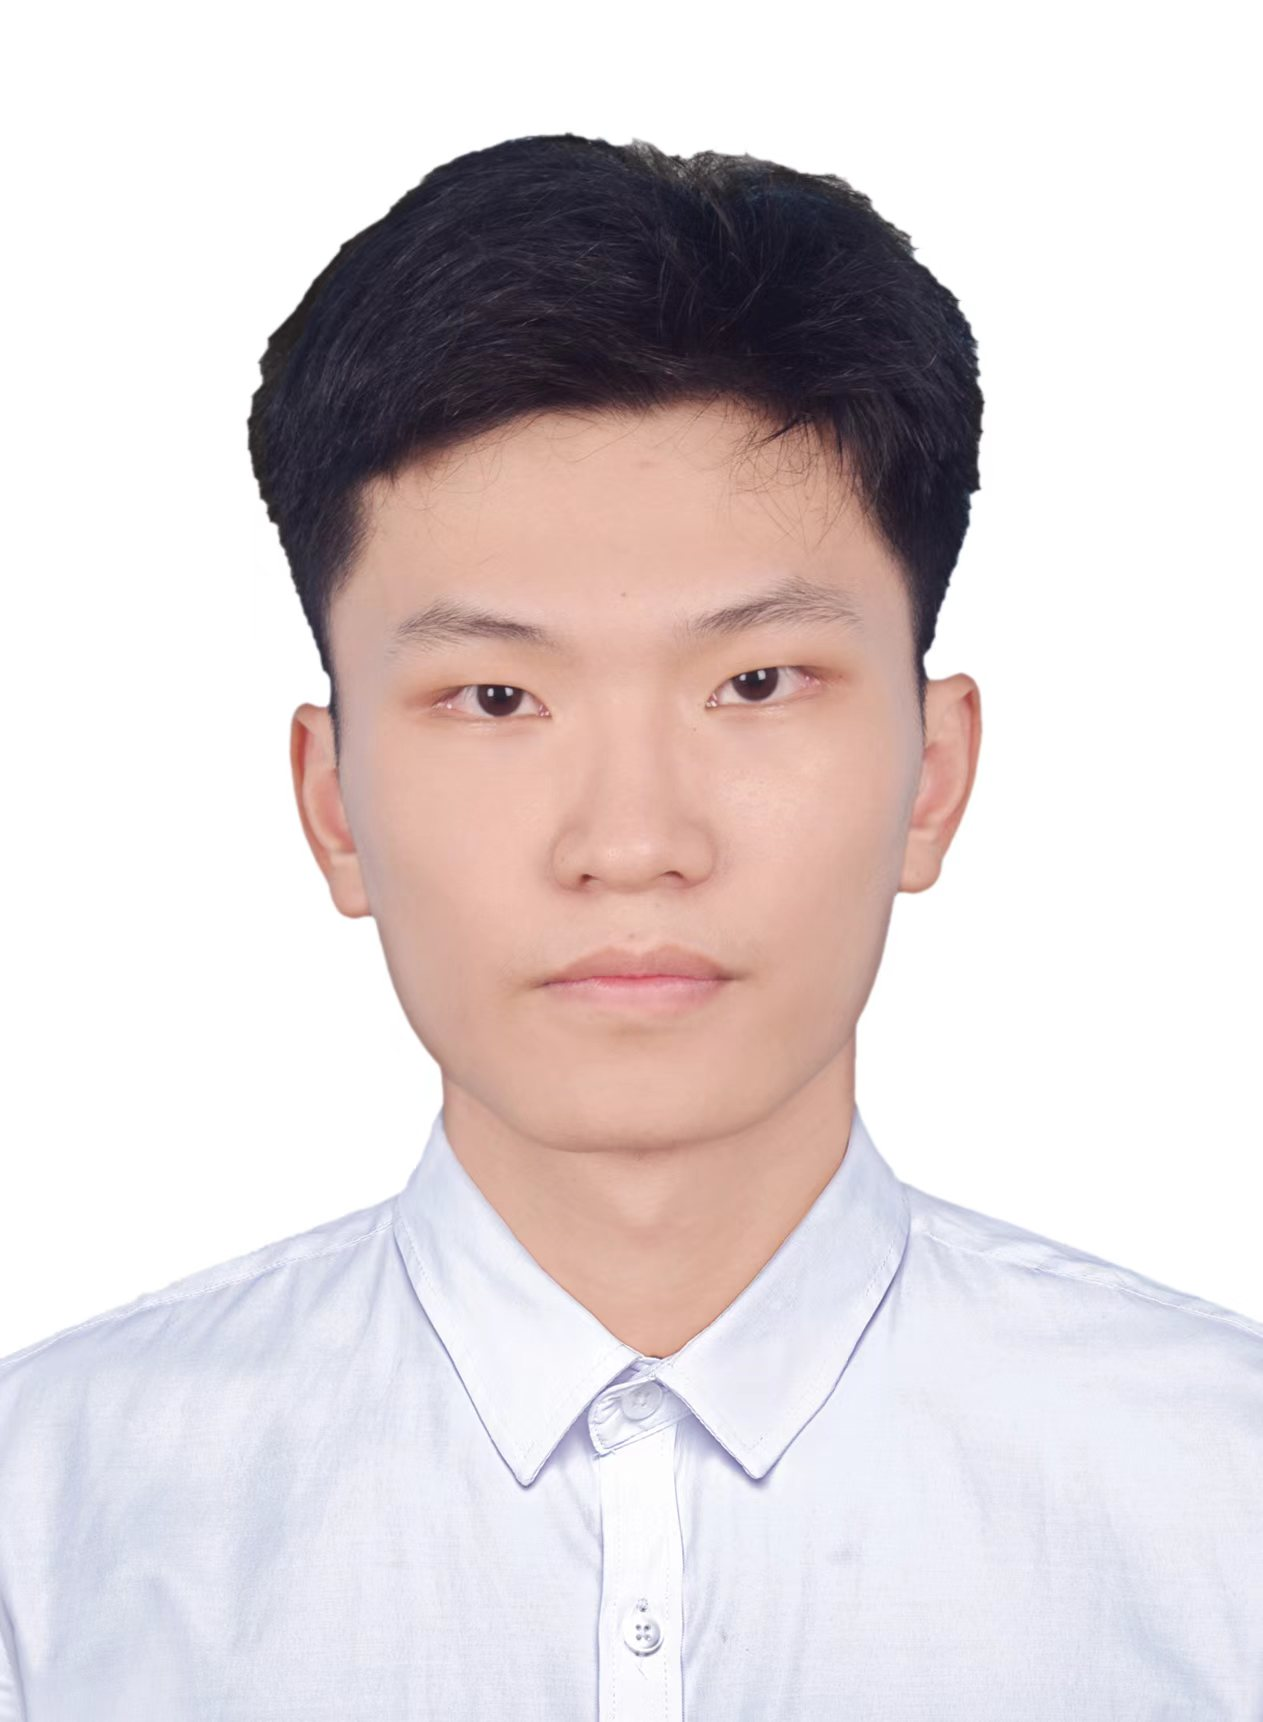
\includegraphics[width=1.3cm,height=1.6cm,keepaspectratio]{刘广裕}
& 刘广裕（202421215123）
& \raggedright
-- 论文撰写、参考文献整理与格式修订\\
-- API 接口规范测试、模拟后端开发与前端性能优化\\
-- 人设文档与表达映射编写、PPT 制作与答辩准备
& 24\% \\
\midrule

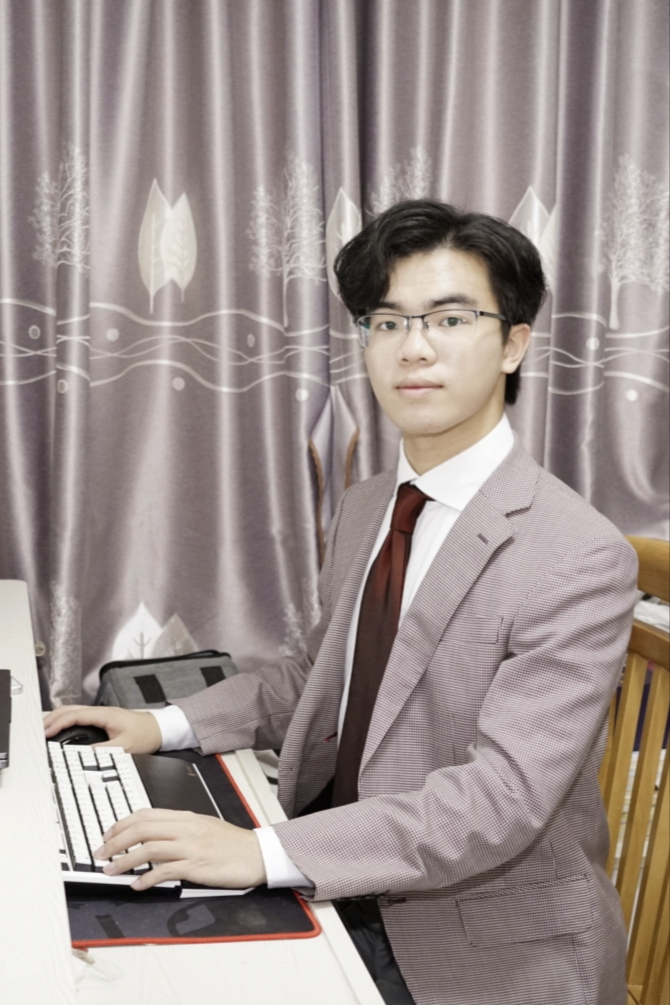
\includegraphics[width=1.3cm,height=1.6cm,keepaspectratio]{杨文博}
& 杨文博（202421215115）
& \raggedright
-- 论文初稿撰写与 LaTeX 排版\\
-- 项目安全访问控制与 LLM 推理优化\\
-- 配置常量管理与代码重构、PPT 制作与答辩准备
& 25\% \\
\midrule

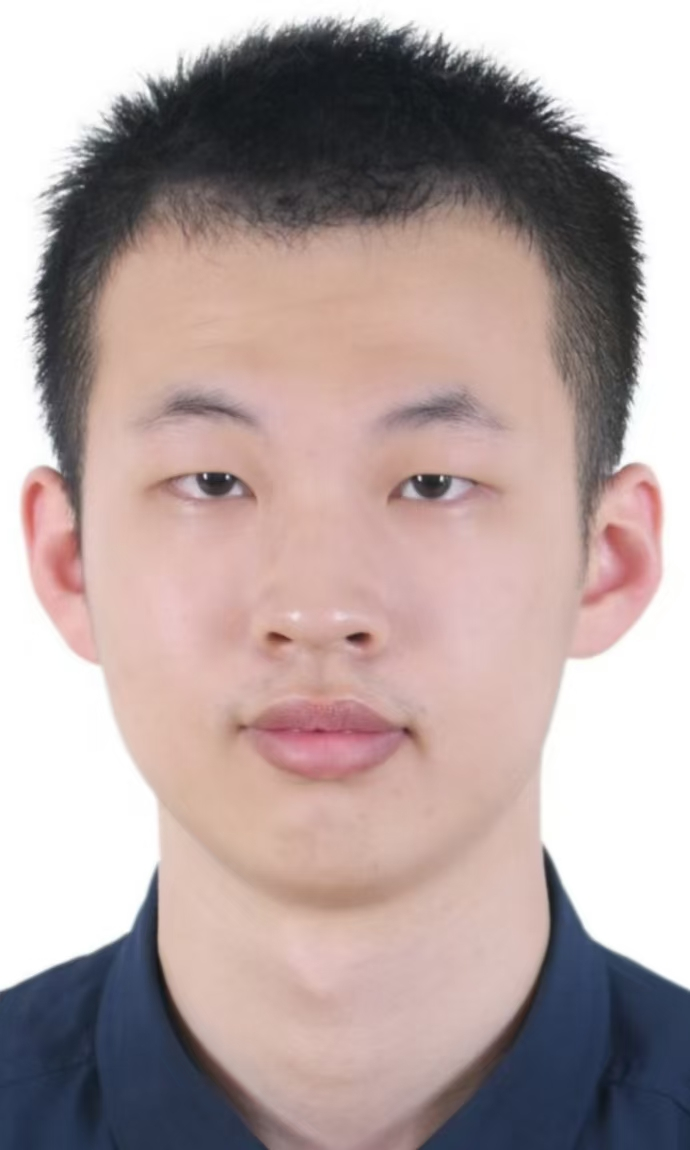
\includegraphics[width=1.3cm,height=1.6cm,keepaspectratio]{温嘉浩}
& 温嘉浩（202421215121）
& \raggedright
-- 后端 Agent 工作流架构设计与 LangGraph 图编排\\
-- 后端文件布局、文档整理与 MiniMax 兼容性优化\\
-- 仓库维护与代码清理、PPT 制作与答辩准备
& 25\% \\
\midrule
\multicolumn{4}{p{\textwidth}}{
\scriptsize\raggedright\textit{注：所有成员贡献占比经小组协商一致确定，合计为 100\%。论文编写由杨文博（初稿与排版）和刘广裕（文献与修订）共同负责，郭凡渊与温嘉浩参与内容审阅。}
} \\
\bottomrule
\end{tabularx}
}
\end{center}

\end{document}
